\documentclass{article}
\usepackage{graphicx} % Required for inserting images
\usepackage{lipsum}
\usepackage[margin=1in, includefoot, includehead]{geometry}
\usepackage{amsmath}
\usepackage{hyperref}
\usepackage[spanish]{babel}
\usepackage{amsfonts}
\usepackage{amssymb}
\usepackage{listings}
\usepackage{xcolor}
\addto\captionsspanish{\renewcommand{\tablename}{Tabla}}
\usepackage[hidelinks]{hyperref}
\usepackage{fancyhdr}
\lstdefinestyle{python}{
    language=Python,
    basicstyle=\ttfamily\footnotesize, % Tipo de letra
    keywordstyle=\color{blue},         % Color para palabras clave
    commentstyle=\color{gray},         % Color para comentarios
    stringstyle=\color{red},           % Color para strings
    breaklines=true,                    % Romper líneas largas
    frame=single,                       % Marco alrededor del código
    backgroundcolor=\color{gray!10},    % Fondo gris claro
    numbers=left,                       % Numeración de líneas a la izquierda
    numberstyle=\tiny\color{gray}       % Estilo de los números de línea
}
\usepackage{tikz}
\pagestyle{fancy}
\fancyhead{}
\usepackage[utf8]{inputenc}      % Para codificación de caracteres
\usepackage{graphicx}            % Para incluir gráficos (opcional pero útil)
\usepackage{amsmath}             % Para mejor soporte de fórmulas matemáticas
\usepackage{float}               % Para usar [H] y controlar la posición de las tablas
\usepackage{array}               % Para columnas con ancho fijo como p{Xcm}
\usepackage{caption}             % Para personalizar captions (opcional)
\fancyfoot{}
\fancyhead[R]{\myTitle}
\fancyfoot[L]{Simulación Numérica}
\fancyfoot[R]{\thepage}
\renewcommand{\footrulewidth}{1pt}
\newcommand{\myTitle}{Informe 2: Examen Parcial}
\newcommand{\myName}{González García, María\\
                    López Rodríguez, Claudia }
\newcommand{\myDate}{\today}

\begin{document}

%PORTADA PRINCIPAL
\begin{titlepage}
    \begin{center}
        
\includegraphics[scale=0.17]{img/UAX.png}\\
        \huge{\textbf{Universidad Alfonso X\\ El Sabio}} \\
        [0.25in] 
        
        \textbf{\Large{Grado en Ingeniería Matemática}}\\
        \Large{Simulación Numérica}\\
    
        \line(1,0){400}\\
        [2mm]
        \textsc{\Large{\myTitle}} \\
        \line(1,0){400} \\
        [1in]
    \end{center}
    \begin{center}
        \textsc{\Large Autor:}	\\
        \myName\\
        [1in]
        \myDate
    \end{center}
\end{titlepage}

%ABSTRACT
\begin{abstract}

En este trabajo se aborda la resolución numérica de la ecuación de calor en dos dimensiones mediante métodos de diferencias finitas. El objetivo principal es obtener tanto la solución transitoria como la solución estacionaria del sistema, considerando condiciones de contorno mixtas: dos lados con temperatura constante y dos lados aislantes.\\

Para la parte transitoria, se empleará un esquema implícito debido a su estabilidad incondicional, lo que permite simular la evolución térmica con pasos de tiempo más grandes sin pérdida de precisión. La ecuación se discretiza mediante diferencias finitas centradas en el espacio y hacia atrás en el tiempo, generando un sistema lineal en cada paso temporal. Este sistema se resolverá utilizando matrices dispersas, lo que reduce significativamente el coste computacional en dominios con alto número de nodos. \\

En cuanto a la solución estacionaria, se aplicará también un método implícito basado en la resolución del sistema en estado estable, es decir, cuando la derivada temporal se anula. Se estudiará el comportamiento del sistema al alcanzar el equilibrio térmico, resolviendo el sistema algebraico resultante con técnicas eficientes apoyadas en matrices dispersas.\\

El trabajo incluirá una descripción teórica de los métodos empleados, así como representaciones gráficas de las soluciones obtenidas, siguiendo una estructura que combine el análisis numérico con una presentación clara y rigurosa de los resultados.

\end{abstract}


%ÍNDICE
\newpage
\tableofcontents

%INTRODUCCIÓN
\newpage
\section{Introducción}

El análisis de fenómenos de transferencia de calor es un problema clásico en el ámbito de la simulación numérica, con aplicaciones relevantes en la ingeniería, la física y otras ciencias aplicadas. En este informe se estudia la evolución de la temperatura en una placa delgada idealizada, sujeta a condiciones de contorno mixtas, a través de la resolución de la ecuación de calor en dos dimensiones. \\

El dominio considerado es el cuadrado unitario definido por $x, y \in (0,1)$, y se analiza su comportamiento térmico a lo largo del tiempo $t > 0$. El modelo matemático que describe este fenómeno está dado por una ecuación de difusión anisotrópica:
$$
\frac{\partial T}{\partial t} - 0.01\left( \frac{\partial^2 T}{\partial x^2} + \frac{\partial^2 T}{\partial y^2} \right) = 0
$$
dónde $T = T(x, y, t)$ representa la temperatura en el punto $(x, y)$ en el instante temporal $t$.\\

La condición inicial prescribe una distribución de temperatura negativa con forma cosenoidal, dada por:
$$
T(x, y, 0) = -50 \cos\left(\frac{\pi x}{2}\right) \cos\left(\frac{\pi y}{2}\right)
$$
Respecto a las condiciones de contorno, se imponen condiciones de tipo Neumann (frontera aislante) en los bordes izquierdo y derecho del dominio:
$$
\frac{\partial T}{\partial x}(0, y, t) = 0, \quad \frac{\partial T}{\partial x}(1, y, t) = 0
$$
y condiciones de tipo Dirichlet (temperatura fija) en los bordes inferior y superior:
$$
T(x, 0, t) = 20, \quad T(x, 1, t) = 50
$$

Este trabajo tiene como finalidad desarrollar una aproximación numérica al problema anterior, abordando tanto su solución transitoria como la solución en estado estacionario. Para ello, se emplearán esquemas de diferencias finitas de tipo implícito. Asimismo, se incorporará la representación de resultados mediante visualizaciones que permitan observar la evolución del campo de temperatura.\\

Desde una perspectiva más técnica, el estudio se enmarca en la formulación y análisis de ecuaciones en derivadas parciales utilizando técnicas de discretización espacio-temporal. La implementación de métodos numéricos permitirá aproximar el comportamiento térmico del sistema con fidelidad, sirviendo como herramienta de validación y análisis cualitativo del fenómeno simulado.


%MÉTODOS Y MODELOS MATEMÁTICOS
\newpage
\section{Métodos y modelos matemáticos.}
En esta sección se presentan los fundamentos matemáticos necesarios para abordar la resolución del problema propuesto. Este se modela mediante una ecuación en derivadas parciales de segundo orden, en un dominio bidimensional acotado $\Omega = (0,1) \times (0,1)$, y en un intervalo temporal $t \in (0, \infty)$. La ecuación representa un proceso de transferencia de calor en un medio homogéneo e isotrópico [\href{https://diposit.ub.edu/dspace/bitstream/2445/211361/1/tfg_iglesias_diaz_angel.pdf}{1}].\\

La formulación general adoptada es la siguiente:
\begin{equation}
    \frac{\partial T}{\partial t} = \alpha \left( \frac{\partial^2 T}{\partial x^2} + \frac{\partial^2 T}{\partial y^2} \right), \quad \text{para } (x, y) \in \Omega,\; t > 0,
\end{equation}

dónde $T = T(x, y, t)$ representa el campo escalar de temperatura en función del tiempo y del espacio, y $\alpha \in \mathbb{R}^+$ es el coeficiente de difusión térmica del material, que mide la capacidad del medio para conducir el calor. Esta formulación se basa en la hipótesis de que el flujo de calor sigue la ley de Fourier, y que la conducción térmica es el único mecanismo relevante para el transporte de energía en el sistema.\\

La ecuación presenta un \textbf{comportamiento isotrópico}, lo que significa que las propiedades del medio son las mismas en todas las direcciones espaciales. En términos prácticos, esto implica que la difusión del calor ocurre con igual intensidad tanto en la dirección del eje $x$ como en la del eje $y$. Matemáticamente, esto se refleja en que los coeficientes que acompañan a las segundas derivadas espaciales son iguales, y físicamente, en que el material no presenta anisotropías estructurales ni variaciones de composición que favorezcan una dirección particular para la propagación térmica.\\

Este tipo de modelo es especialmente relevante en contextos dónde el medio es continuo, homogéneo y carece de discontinuidades o heterogeneidades a escala macroscópica. Es aplicable, por ejemplo, a materiales sólidos uniformes, como metales bien pulidos o geles isotrópicos, en los que la temperatura se disemina suavemente desde zonas calientes hacia zonas frías, siguiendo una distribución que depende únicamente del gradiente térmico y no de la orientación espacial [\href{https://es.wikipedia.org/wiki/Ecuaci%C3%B3n_del_calor}{2}].

\begin{enumerate}
    \item \textbf{Solución transitoria} (véase Sección~\ref{subsec:st})\textbf{:} La solución transitoria describe la \textbf{evolución dinámica del sistema térmico desde una condición inicial no trivial}. Permite analizar cómo se redistribuye la temperatura en el dominio conforme avanza el tiempo, hasta alcanzar una configuración estable. Para su estudio se emplean esquemas numéricos de discretización espacio-temporal, cuya elección debe considerar criterios de estabilidad, consistencia y convergencia.

    \item \textbf{Solución estacionaria} (véase Sección~\ref{subsec:se})\textbf{:} La solución estacionaria corresponde al régimen en el que l\textbf{as variaciones temporales se anulan}, es decir, cuando el sistema alcanza el equilibrio térmico. Matemáticamente, se obtiene imponiendo $\partial T/\partial t = 0$, lo que reduce la ecuación a una forma puramente espacial. El análisis estacionario es esencial para caracterizar el comportamiento térmico permanente del sistema, independiente del estado inicial.
\end{enumerate}

Aunque el enunciado requiere implementar únicamente un método por cada régimen —transitorio y estacionario—, se expondrán de forma sucinta otras metodologías relevantes (explícitas, implícitas, iterativas) con el fin de proporcionar un marco de referencia sólido y facilitar la comprensión del enfoque adoptado. El desarrollo principal del presente trabajo se centrará en los métodos implícitos con formulación matricial dispersa (\textit{sparse}), dada su eficiencia computacional y su adecuación a problemas de gran dimensión.

\newpage
\subsection{Solución Transitoria.}
\label{subsec:st}
El análisis transitorio permite estudiar cómo \textbf{evoluciona la distribución de temperatura} en el dominio a lo largo del tiempo, a partir de una \textbf{condición inicial} determinada y bajo unas \textbf{condiciones de contorno} específicas. Se trata, por tanto, de un fenómeno \textbf{dinámico} cuya descripción requiere la \textbf{discretización} tanto de las \textbf{variables espaciales} como de la \textbf{variable temporal}.\\

Desde el punto de vista numérico, la simulación de este tipo de problemas puede llevarse a cabo mediante distintos esquemas basados en \textbf{diferencias finitas}. Entre los más comunes se encuentran el \textbf{método explícito}, el \textbf{método implícito} y sus variantes optimizadas mediante el uso de \textbf{matrices dispersas}. Cada uno de estos enfoques presenta ventajas e inconvenientes en términos de estabilidad, precisión y coste computacional.\\

A continuación, se presentan brevemente estos métodos con el objetivo de ofrecer un \textbf{marco teórico comparativo} y facilitar la comprensión del enfoque seleccionado. Aunque en este trabajo se implementará únicamente el \textbf{método implícito con matrices sparse}, se incluyen los demás para \textbf{contextualizar adecuadamente} la estrategia adoptada [\href{https://webs.um.es/gustavo.garrigos/tfg/Milonga_TFG_sept2020.pdf}{3}].

\subsubsection{Método Explícito.}
\label{subsubsec:me}
El \textbf{método explícito} es una técnica numérica basada en esquemas de diferencias finitas, comúnmente utilizada para resolver \textbf{ecuaciones en derivadas parciales de tipo parabólico}, como la ecuación del calor. Su principal ventaja radica en su \textbf{simplicidad computacional}: permite calcular la solución en el instante siguiente a partir de los valores ya conocidos, sin necesidad de resolver sistemas de ecuaciones lineales.\\

En este caso, se desea resolver la ecuación del calor en dos dimensiones:
\begin{equation}
\label{eq:or}
    \frac{\partial T}{\partial t} = \alpha \left( \frac{\partial^2 T}{\partial x^2} + \frac{\partial^2 T}{\partial y^2} \right)
\end{equation}
dónde $T(x, y, t)$ representa la distribución de temperatura en el dominio, y $\alpha$ es el coeficiente de difusión térmica. Se considera una malla \textbf{cuadrada uniforme}, con paso espacial $h$ en ambas direcciones y paso temporal constante $\Delta t$. El valor aproximado de la solución en el nodo espacial $(x_i, y_j)$ en el instante $t^n = n\Delta t$ se denota por $T_{i,j}^n$ [\href{https://personales.upv.es/dginesta/docencia/posgrado/prac_intro_edps.pdf}{4}].

\paragraph{Deducción paso a paso del esquema explícito.}
Consideramos la ecuación con derivada temporal de primer orden y signo positivo en los términos espaciales. Suponiendo una malla cuadrada, es decir, $\Delta x = \Delta y = h$, se aproximan las derivadas mediante diferencias finitas centradas:

\begin{itemize}
    \item Derivada temporal:
    $$
    \frac{\partial T}{\partial t}(x_i, y_j, t^n) \approx \frac{T_{i,j}^{n+1} - T_{i,j}^{n}}{\Delta t}
    $$
    \item Derivadas espaciales:
    $$
    \frac{\partial^2 T}{\partial x^2}(x_i, y_j, t^n) \approx \frac{T_{i+1,j}^n - 2T_{i,j}^n + T_{i-1,j}^n}{h^2}, \quad
    \frac{\partial^2 T}{\partial y^2}(x_i, y_j, t^n) \approx \frac{T_{i,j+1}^n - 2T_{i,j}^n + T_{i,j-1}^n}{h^2}
    $$
\end{itemize}

\noindent Sustituyendo estas expresiones en la ecuación original (Ver Ecuación~\ref{eq:or}):
\begin{equation}
    \frac{T_{i,j}^{n+1} - T_{i,j}^{n}}{\Delta t}
    = \alpha \left(
    \frac{T_{i+1,j}^n - 2T_{i,j}^n + T_{i-1,j}^n}{h^2}
    +
    \frac{T_{i,j+1}^n - 2T_{i,j}^n + T_{i,j-1}^n}{h^2}
    \right)
\end{equation}

$$
T_{i,j}^{n+1} - T_{i,j}^{n}
= \frac{\alpha \Delta t}{h^2} \left[
(T_{i+1,j}^n + T_{i-1,j}^n - 2T_{i,j}^n)
+
(T_{i,j+1}^n + T_{i,j-1}^n - 2T_{i,j}^n)
\right]
$$

\noindent Definimos el parámetro $\lambda = \frac{\alpha \Delta t}{h^2}$ y obtenemos finalmente el esquema explícito general:

$$
T_{i,j}^{n+1} = T_{i,j}^{n} + \lambda \left(
T_{i+1,j}^n + T_{i-1,j}^n + T_{i,j+1}^n + T_{i,j-1}^n - 4T_{i,j}^n
\right)
$$

Este esquema explícito permite avanzar la solución en el tiempo utilizando exclusivamente valores conocidos del instante anterior. Su precisión es de segundo orden en espacio y primer orden en tiempo. La estabilidad del método, no obstante, está condicionada al valor de $\lambda$, como se explicará en el siguiente apartado.

\paragraph{Condición de estabilidad (CFL).} El método explícito es \textbf{condicionalmente estable}, lo que significa que solo garantiza soluciones numéricamente estables si se cumple una restricción sobre el parámetro $\lambda$. En el caso bidimensional con malla cuadrada, debe cumplirse:
$$
\lambda < \frac{1}{2} \quad \Rightarrow \quad \Delta t < \frac{h^2}{2\alpha}
$$
Cuando esta condición no se satisface, el método puede generar errores crecientes con cada paso de tiempo, llevando a soluciones inestables y físicamente incoherentes.

\paragraph{Tratamiento de fronteras.} En los bordes del dominio, algunos nodos vecinos requeridos por el esquema (por ejemplo, $T_{i-1,j}$ o $T_{i,j+1}$) pueden no existir dentro de la malla. Para resolver este problema, se aplican las \textbf{condiciones de contorno} adecuadas:

\begin{itemize}
    \item Si la condición es \textbf{Dirichlet}, se impone directamente el valor: $T(x=0, y, t) = 20 \Rightarrow T_{0,j}^n = 20$
    \item Si es una condición \textbf{Neumann}, se sustituye usando una diferencia centrada:
    $\left. \frac{\partial T}{\partial x} \right|_{x=1} = 0 \Rightarrow T_{N+1,j}^n = T_{N-1,j}^n$
\end{itemize}

\noindent Esto permite evaluar correctamente la fórmula sin necesidad de extrapolar valores fuera del dominio definido.

\paragraph{Ventajas y limitaciones.} A continuación, se presentan las principales ventajas y limitaciones del método explícito en el contexto de ecuaciones en derivadas parciales de segundo orden:

\begin{table}[H]
\centering
\begin{tabular}{|p{6.5cm}|p{6.5cm}|}
\hline
\textbf{Ventajas} & \textbf{Limitaciones} \\
\hline
Fácil de implementar. & Requiere paso de tiempo muy pequeño. \\
\hline
Bajo costo computacional por paso. & Estabilidad sujeta a condición restrictiva. \\
\hline
Permite seguir la evolución temporal. & Difícil de aplicar en geometrías complejas. \\
\hline
Ideal para mallas regulares y problemas simples. & Tratamiento especial en el primer paso. \\
\hline
\end{tabular}
\caption{Ventajas y limitaciones del método explícito.}
\end{table}

Concluimos que es ideal para problemas sencillos o con geometrías regulares, en aplicaciones de mayor escala o precisión se suele recurrir a métodos implícitos, que permiten mayores pasos de tiempo sin comprometer la estabilidad.

\subsubsection{Método Implícito.}
\label{subsubsec:mi}
El \textbf{método implícito} es una técnica de resolución numérica que consiste en evaluar las derivadas espaciales en el instante temporal futuro $t^{n+1}$, en lugar del presente $t^n$, como se hace en el método explícito (véase Sección~\ref{subsubsec:me}). Esta característica implica que los valores desconocidos $T_{i,j}^{n+1}$ aparecen en ambos lados de la ecuación, lo que obliga a resolver un sistema lineal acoplado en cada paso temporal. Aunque su implementación es más compleja, este enfoque ofrece mayor estabilidad numérica y permite utilizar pasos de tiempo más grandes sin comprometer la convergencia [\href{https://www.ugr.es/~prodelas/ftp/ETSICCP/Resoluci%F3nNum%E9ricaEDPs.pdf}{5}].

\paragraph{Deducción paso a paso del esquema implícito.} Consideramos la ecuación del calor en 2D:
\begin{equation}
    \frac{\partial T}{\partial t} = \alpha \left( \frac{\partial^2 T}{\partial x^2} + \frac{\partial^2 T}{\partial y^2} \right)
\end{equation}

Se discretiza el dominio con una malla cuadrada de paso $h$ y un paso de tiempo $\Delta t$, y se denota $T_{i,j}^n \approx T(x_i, y_j, t^n)$. Usamos las siguientes diferencias finitas de segundo orden:
\begin{itemize}
    \item Derivada temporal:
    $$
    \frac{\partial T}{\partial t}(x_i, y_j, t^n) \approx \frac{T_{i,j}^{n+1} - T_{i,j}^{n}}{\Delta t}
    $$
    \item Derivadas espaciales evaluadas en $t^{n+1}$ (implícito):
    $$
    \frac{\partial^2 T}{\partial x^2} \approx \frac{T_{i+1,j}^{n+1} - 2T_{i,j}^{n+1} + T_{i-1,j}^{n+1}}{h^2}, \quad
    \frac{\partial^2 T}{\partial y^2} \approx \frac{T_{i,j+1}^{n+1} - 2T_{i,j}^{n+1} + T_{i,j-1}^{n+1}}{h^2}
    $$
\end{itemize}
Sustituimos en la ecuación, multiplicamos por $\Delta t$ y definimos $\lambda = \frac{\alpha \Delta t}{h^2}$:
$$
T_{i,j}^{n+1} - T_{i,j}^{n} = 
\lambda \left(
T_{i+1,j}^{n+1} + T_{i-1,j}^{n+1} + T_{i,j+1}^{n+1} + T_{i,j-1}^{n+1} - 4T_{i,j}^{n+1}
\right) \xrightarrow[]{}
$$

$$
T_{i,j}^{n+1} - \lambda \left(
T_{i+1,j}^{n+1} + T_{i-1,j}^{n+1} + T_{i,j+1}^{n+1} + T_{i,j-1}^{n+1}
\right)
+ 4\lambda T_{i,j}^{n+1}
= T_{i,j}^{n}
$$

Reordenando los términos, y considerando que, como se ha señalado previamente, el método implícito se fundamenta en la evaluación de los términos espaciales en el instante temporal futuro $n+1$, se obtiene la siguiente expresión:

\begin{equation}
    \left(1 + 4\lambda \right) T_{i,j}^{n+1} 
    - \lambda T_{i+1,j}^{n+1}
    - \lambda T_{i-1,j}^{n+1}
    - \lambda T_{i,j+1}^{n+1}
    - \lambda T_{i,j-1}^{n+1}
    = T_{i,j}^{n}
\end{equation}

\paragraph{Estructura de la matriz $A$ para una malla $N \times N$.} Aplicando el método implícito sobre una malla de tamaño $N \times N$ se obtiene, en cada paso temporal, un sistema lineal de la forma:

\begin{equation}
    A \cdot \vec{T}^{\,n+1} = \vec{T}^{\,n}
    \quad \text{con } A \in \mathbb{R}^{N^2 \times N^2} 
\end{equation}
Cada nodo interior del dominio se numera lexicográficamente como:
$$
k = i + j \cdot N \quad \text{con } i, j = 0, \dots, N-1
$$

\paragraph{Lógica de construcción de la matriz $A$.} La matriz $A$ es simétrica, dispersa y presenta como máximo 5 elementos no nulos por fila. Para cada fila $k$, que representa la ecuación asociada al nodo $(i,j)$, se construye del siguiente modo:

\begin{itemize}
    \item $A_{k,k} = 1 + 4\lambda$: Contribución del nodo central.
    \item $A_{k,k-1} = A_{k,k+1} = -\lambda$: Si $k-1$ y $k+1$ están en la misma fila (evitando saltos de fila).
    \item $A_{k,k-N} = A_{k,k+N} = -\lambda$: Si los nodos superior/inferior están dentro del dominio.
\end{itemize}
Este patrón corresponde al esquema de 5 puntos centrado para la ecuación del calor, y permanece constante en el tiempo.

$$
\begin{bmatrix}
1+4\lambda & -\lambda & 0 & \cdots & -\lambda & 0 & \cdots \\
-\lambda & 1+4\lambda & -\lambda & \cdots & 0 & -\lambda & \cdots \\
0 & -\lambda & 1+4\lambda & \cdots & 0 & 0 & \cdots \\
\vdots & \vdots & \vdots & \ddots & \vdots & \vdots & \ddots \\
-\lambda & 0 & 0 & \cdots & 1+4\lambda & -\lambda & \cdots \\
0 & -\lambda & 0 & \cdots & -\lambda & 1+4\lambda & \cdots \\
\vdots & \vdots & \vdots & \ddots & \vdots & \vdots & \ddots
\end{bmatrix}_{N^2 \times N^2}
\cdot
\begin{bmatrix}
T_{0,0}^{n+1} \\
T_{1,0}^{n+1} \\
\vdots \\
T_{N-1,0}^{n+1} \\
T_{0,1}^{n+1} \\
\vdots \\
T_{N-1,N-1}^{n+1}
\end{bmatrix}
=
\begin{bmatrix}
T_{0,0}^{n} \\
T_{1,0}^{n} \\
\vdots \\
T_{N-1,0}^{n} \\
T_{0,1}^{n} \\
\vdots \\
T_{N-1,N-1}^{n}
\end{bmatrix}
\quad \text{con } \lambda = \frac{\alpha \Delta t}{h^2}
$$

\paragraph{Ejemplo: Sistema resultante para una malla $3 \times 3$.} Para ilustrar la construcción del sistema lineal, consideramos una malla cuadrada de $3 \times 3$ nodos interiores. Esto genera un total de $9$ incógnitas en cada paso temporal. Usando el esquema implícito, se obtiene el sistema lineal:

$$
A \cdot \vec{T}^{\,n+1} = \vec{T}^{\,n}, \quad A \in \mathbb{R}^{9 \times 9}
$$

Los nodos se numeran de izquierda a derecha y de abajo hacia arriba (orden fila por fila), según la siguiente tabla:

\begin{figure}[H]
\centering
\begin{minipage}[c]{0.45\textwidth}
\centering
\begin{tabular}{|c|c|c|}
\hline
Índice $k$ & Coordenada $(i,j)$ & Variable \\
\hline
0 & $(0,0)$ & $T_0 = T_{0,0}$ \\
1 & $(1,0)$ & $T_1 = T_{1,0}$ \\
2 & $(2,0)$ & $T_2 = T_{2,0}$ \\
3 & $(0,1)$ & $T_3 = T_{0,1}$ \\
4 & $(1,1)$ & $T_4 = T_{1,1}$ \\
5 & $(2,1)$ & $T_5 = T_{2,1}$ \\
6 & $(0,2)$ & $T_6 = T_{0,2}$ \\
7 & $(1,2)$ & $T_7 = T_{1,2}$ \\
8 & $(2,2)$ & $T_8 = T_{2,2}$ \\
\hline
\end{tabular}
\captionof{table}{Asociación entre índices, coordenadas y variables de los nodos.}
\end{minipage}
\hspace{0.5cm} % Espacio pequeño entre tabla y figura
\begin{minipage}[c]{0.5\textwidth}
\centering
\begin{tikzpicture}[scale=1.4, every node/.style={font=\small}]

% Nodos
\foreach \i in {0,1,2} {
    \foreach \j in {0,1,2} {
        \draw[fill=white] (\i,\j) circle(2pt);
    }
}

% Conexiones horizontales
\foreach \j in {0,1,2} {
    \foreach \i in {0,1} {
        \draw (\i,\j) -- (\i+1,\j);
    }
}

% Conexiones verticales
\foreach \i in {0,1,2} {
    \foreach \j in {0,1} {
        \draw (\i,\j) -- (\i,\j+1);
    }
}

% Etiquetas
\foreach \i/\j/\k in {
    0/0/0, 1/0/1, 2/0/2,
    0/1/3, 1/1/4, 2/1/5,
    0/2/6, 1/2/7, 2/2/8} {
    \node[above right] at (\i,\j) {$T_{\k}$};
    \node[below left] at (\i,\j) {$(\i,\j)$};
}

\end{tikzpicture}
\vspace{0.2mm}
\captionof{figure}{Mallado $3 \times 3$ con numeración lexicográfica.}
\end{minipage}
\end{figure}

La matriz $A$ tiene estructura dispersa derivada del esquema de 5 puntos, y los vectores de incógnitas y segundo miembro se expresan así:

$$
\begin{bmatrix}
1+4\lambda & -\lambda & 0         & -\lambda & 0         & 0         & 0         & 0         & 0 \\
-\lambda   & 1+4\lambda & -\lambda & 0         & -\lambda & 0         & 0         & 0         & 0 \\
0         & -\lambda & 1+4\lambda & 0         & 0         & -\lambda & 0         & 0         & 0 \\
-\lambda   & 0         & 0         & 1+4\lambda & -\lambda & 0         & -\lambda & 0         & 0 \\
0         & -\lambda & 0         & -\lambda & 1+4\lambda & -\lambda & 0         & -\lambda & 0 \\
0         & 0         & -\lambda & 0         & -\lambda & 1+4\lambda & 0         & 0         & -\lambda \\
0         & 0         & 0         & -\lambda & 0         & 0         & 1+4\lambda & -\lambda & 0 \\
0         & 0         & 0         & 0         & -\lambda & 0         & -\lambda & 1+4\lambda & -\lambda \\
0         & 0         & 0         & 0         & 0         & -\lambda & 0         & -\lambda & 1+4\lambda
\end{bmatrix}
\cdot
\begin{bmatrix}
T_0^{n+1} \\
T_1^{n+1} \\
T_2^{n+1} \\
T_3^{n+1} \\
T_4^{n+1} \\
T_5^{n+1} \\
T_6^{n+1} \\
T_7^{n+1} \\
T_8^{n+1}
\end{bmatrix}
=
\begin{bmatrix}
T_0^n \\
T_1^n \\
T_2^n \\
T_3^n \\
T_4^n \\
T_5^n \\
T_6^n \\
T_7^n \\
T_8^n
\end{bmatrix}
\quad \text{con } \lambda = \frac{\alpha \Delta t}{h^2}
$$
Esta matriz se genera a partir del esquema implícito aplicado a la ecuación del calor en 2D utilizando una malla de $3 \times 3$ nodos interiores. Cada fila $k$ del sistema corresponde a un nodo $(i,j)$ numerado lexicográficamente como $k = i + j \cdot 3$.

\begin{itemize}
    \item El valor diagonal $1 + 4\lambda$ representa la contribución del nodo central $T_{i,j}^{n+1}$.
    \item Los coeficientes $-\lambda$ fuera de la diagonal reflejan la conexión con los cuatro vecinos inmediatos:
    \begin{itemize}
        \item $k \pm 1$ son los vecinos en la misma fila (izquierda y derecha), respetando que no haya salto de fila.
        \item $k \pm 3$ son los vecinos en la fila superior o inferior (verticalmente), siendo $N = 3$ el número de nodos por fila.
    \end{itemize}
    \item Los ceros indican que el nodo $k$ no está conectado con otros nodos fuera de su vecindad directa.
\end{itemize}
Este sistema se puede resolver en cada paso temporal utilizando técnicas numéricas eficientes, especialmente si se representa la matriz $A$ en formato disperso (\texttt{CSR} o \texttt{COO}) (ver Sección~\ref{subsubsec:sparse}).

\paragraph{Tratamiento de condiciones de contorno.} Al aplicar un método numérico en un dominio espacial finito, es imprescindible incorporar adecuadamente las \textbf{condiciones de contorno}, ya que en los nodos de los bordes algunas de las derivadas espaciales no pueden calcularse directamente con el esquema habitual por falta de vecinos exteriores. Estas condiciones definen el comportamiento del sistema en sus límites y permiten cerrar correctamente el sistema de ecuaciones. En este trabajo se imponen dos tipos de condiciones:

\begin{itemize}
    \item \textbf{Condiciones de Dirichlet:} Prescriben directamente el valor de la temperatura en los bordes del dominio. Es decir, se fijan directamente los valores en la solución. En este caso, se fijan:
    $$
    T(x, 0, t) = 20 \quad \text{y} \quad T(x, 1, t) = 50 
    \quad \Longrightarrow \quad 
    T_{i,0}^n = 20, \quad T_{i,N+1}^n = 50 \quad \forall\, n \in \mathbb{N}
    $$
    Estas condiciones se aplican de forma directa en la malla, sustituyendo los valores correspondientes en el vector de incógnitas por los valores prescritos, y ajustando el segundo miembro si es necesario.

    \item \textbf{Condiciones de Neumann:} Imponen una derivada normal nula, es decir, que no hay flujo térmico a través del borde. En el esquema de diferencias finitas, esto se traduce en sustituir el valor fuera del dominio por una reflexión del valor interior. Es decir, se sustituyen los nodos ficticios por expresiones en términos de nodos interiores. En nuestro caso:
    $$
    \begin{aligned}
    &\left. \frac{\partial T}{\partial x} \right|_{x=0} = 0 
    \quad \Longrightarrow \quad 
    \frac{T_{1,j}^n - T_{-1,j}^n}{2h} = 0 
    \quad \Longrightarrow \quad 
    T_{-1,j}^n = T_{1,j}^n, \\
    &\left. \frac{\partial T}{\partial x} \right|_{x=1} = 0 
    \quad \Longrightarrow \quad 
    \frac{T_{N+1,j}^n - T_{N-1,j}^n}{2h} = 0 
    \quad \Longrightarrow \quad 
    T_{N+1,j}^n = T_{N-1,j}^n 
    \qquad \forall\, n \in \mathbb{N}
    \end{aligned}
    $$

    Estas sustituciones permiten evaluar el esquema numérico en los nodos frontera sin necesidad de acceder a nodos fuera del dominio real. Se basan en la simetría de la derivada nula respecto al borde [\href{https://www.dmae.upct.es/~paredes/calcnum/apuntes/apuntes_tema_7.pdf}{6}].
\end{itemize}

\paragraph{Condición de estabilidad.} El método implícito, a diferencia del explícito, es \textbf{estable incondicionalmente} para muchos problemas lineales, lo que significa que no requiere restricciones sobre $\Delta t$ ni sobre el parámetro $\lambda$. Esta propiedad es especialmente útil, dónde el método explícito podría presentar inestabilidad incluso con pasos de tiempo muy pequeños.

\paragraph{Ventajas y limitaciones.} A continuación, se resumen las principales fortalezas y debilidades del método implícito aplicado a la resolución de ecuaciones en derivadas parciales de segundo orden:

\begin{table}[H]
\centering
\begin{tabular}{|p{6.5cm}|p{6.5cm}|}
\hline
\textbf{Ventajas} & \textbf{Limitaciones} \\
\hline
Estabilidad incondicional para ecuaciones lineales. & Requiere resolver un sistema lineal en cada paso. \\
\hline
Permite emplear pasos de tiempo grandes. & Mayor complejidad de implementación. \\
\hline
Adecuado para ecuaciones con comportamiento anisotrópico. & Mayor coste computacional por iteración. \\
\hline
Compatible con estructuras matriciales sparse. & Tratamiento de condiciones de contorno más delicado. \\
\hline
\end{tabular}
\caption{Ventajas y limitaciones del método implícito.}
\end{table}

\newpage
\subsubsection{Método Implícito con Matrices Sparse.}
\label{subsubsec:sparse}
Como se ha expuesto en el apartado anterior, la aplicación del método implícito a ecuaciones parabólicas como la del calor genera, en cada paso temporal, un sistema lineal acoplado de gran tamaño cuya matriz presenta una estructura muy regular pero altamente dispersa. A fin de resolver dicho sistema de forma eficiente y escalable, es necesario adoptar representaciones optimizadas conocidas como \textbf{estructuras sparse} o matrices dispersas.

\paragraph{Formulación matricial del sistema.}

Al aplicar diferencias finitas centradas en espacio y hacia adelante en tiempo, se obtiene una ecuación de la forma:
$$
(1 + 4\lambda) T_{i,j}^{n+1}
- \lambda T_{i+1,j}^{n+1}
- \lambda T_{i-1,j}^{n+1}
- \lambda T_{i,j+1}^{n+1}
- \lambda T_{i,j-1}^{n+1}
= T_{i,j}^{n}
$$
dónde $\lambda = \frac{\alpha \Delta t}{h^2}$. Esta expresión se genera para cada nodo interior del dominio discreto, y se traduce a una fila del sistema lineal:
$$
A \cdot \vec{T}^{\,n+1} = \vec{T}^n
$$
La matriz $A \in \mathbb{R}^{N^2 \times N^2}$ posee una estructura dispersa: cada fila contiene como máximo cinco coeficientes no nulos (el nodo central más sus cuatro vecinos inmediatos), lo que justifica el uso de estructuras de almacenamiento eficientes.

\paragraph{Construcción estructurada de la matriz.} Se considera una malla regular de $N_x \times N_y$ nodos interiores. Cada nodo $(i,j)$ se numera como:

$$
k = i + j \cdot N_x, \quad \text{con } 0 \leq i < N_x, \; 0 \leq j < N_y
$$

y da lugar a una ecuación de la forma:

\begin{itemize}
    \item $A_{k,k} = 1 + 4\lambda$: Nodo central.
    \item $A_{k,k \pm 1} = -\lambda$: Nodos vecinos en la misma fila (izquierda y derecha).
    \item $A_{k,k \pm N_x} = -\lambda$: Nodos vecinos en columnas adyacentes (arriba y abajo).
\end{itemize}

Este patrón corresponde al esquema clásico de cinco puntos, aplicado a todos los nodos interiores del dominio.

\paragraph{Tratamiento de condiciones de contorno.}

En los bordes del dominio se aplican condiciones de contorno específicas:

\begin{itemize}
    \item En las fronteras horizontales ($y = 0$ y $y = 1$), se imponen condiciones de \textbf{Dirichlet}. Esto se traduce en la fijación directa de los valores del vector solución $\vec{T}^{n+1}$ en los nodos de dichas líneas y la modificación del segundo miembro en consecuencia.
    $$
    T(x, 0, t) = 20 \quad \text{y} \quad T(x, 1, t) = 50 
    \quad \Longrightarrow \quad 
    T_{i,0}^n = 20, \quad T_{i,N+1}^n = 50 \quad \forall\, n \in \mathbb{N}
    $$
    \item En las fronteras verticales ($x = 0$ y $x = 1$), se aplican condiciones de \textbf{Neumann homogéneas} (derivada nula), que implican que la temperatura no varía en la dirección normal al borde. Esto se implementa duplicando el coeficiente del nodo interior más cercano.
    $$
    \begin{aligned}
    &\left. \frac{\partial T}{\partial x} \right|_{x=0} = 0 
    \quad \Longrightarrow \quad 
    \frac{T_{1,j}^n - T_{-1,j}^n}{2h} = 0 
    \quad \Longrightarrow \quad 
    T_{-1,j}^n = T_{1,j}^n, \\
    &\left. \frac{\partial T}{\partial x} \right|_{x=1} = 0 
    \quad \Longrightarrow \quad 
    \frac{T_{N+1,j}^n - T_{N-1,j}^n}{2h} = 0 
    \quad \Longrightarrow \quad 
    T_{N+1,j}^n = T_{N-1,j}^n 
    \qquad \forall\, n \in \mathbb{N}
    \end{aligned}
    $$
\end{itemize}

\paragraph{Representación de la matriz: Estructuras sparse.} En el contexto del método implícito aplicado a la ecuación del calor en 2D, la formulación discreta da lugar a un sistema lineal acoplado cuya matriz $A \in \mathbb{R}^{N^2 \times N^2}$ presenta una estructura altamente dispersa: cada fila contiene como máximo cinco elementos no nulos (nodo central y cuatro vecinos inmediatos). Al aumentar la resolución espacial, el número de nodos crece cuadráticamente, pero el número de elementos no nulos lo hace linealmente. Esto hace inviable el uso de representaciones densas, tanto por coste computacional como por memoria.\\

Para afrontar esta limitación, se emplean formatos de almacenamiento disperso que permiten representar únicamente los valores útiles de la matriz. Los más utilizados en contextos científicos son el formato \textbf{COO (Coordinate List)} y el \textbf{CSR (Compressed Sparse Row)}. Ambos ofrecen una forma compacta y eficiente de representar y operar con matrices dispersas, y su uso conjunto permite una construcción y resolución optimizadas del sistema.

\paragraph{Flujo general de uso: COO \textrightarrow{} CSR.}

El flujo habitual de implementación se basa en las siguientes etapas:

\begin{enumerate}
    \item \textbf{Construcción de la matriz en formato \texttt{COO}:} Se recorre cada nodo interior del dominio y se agregan las contribuciones correspondientes (central y vecinos) en forma de tuplas \texttt{(fila, columna, valor)}. Este formato es flexible y permite ensamblar la matriz sin necesidad de conocer previamente la estructura de filas.

    \item \textbf{Conversión a formato \texttt{CSR}:} Una vez completada la matriz, se transforma a \texttt{CSR}, lo que permite recorrer directamente las filas y aplicar métodos iterativos o solvers directos eficientes. La compresión por filas elimina la necesidad de operar sobre ceros y reduce significativamente el coste computacional.

    \item \textbf{Resolución del sistema:} El sistema lineal $A \cdot \vec{T}^{n+1} = \vec{b}$ se resuelve utilizando técnicas especializadas en matrices sparse, como factorización LU dispersa o métodos iterativos acelerados, garantizando estabilidad y escalabilidad.
\end{enumerate}

\paragraph{Formato COO (Coordinate List).} 
\phantomsection
\label{par:coo} El formato \texttt{COO} representa una matriz dispersa mediante tres vectores:
\begin{itemize}
    \item \texttt{data}: Contiene los valores no nulos.
    \item \texttt{row}: Contiene el índice de fila de cada entrada.
    \item \texttt{col}: Contiene el índice de columna correspondiente.
\end{itemize}
\paragraph{Formato CSR (Compressed Sparse Row).} El formato \texttt{CSR} reorganiza los datos para favorecer un acceso eficiente por filas, y se compone de:
\label{paragraph:csr}
\begin{itemize}
    \item \texttt{data}: Almacena todos los elementos no nulos de la matriz, ordenados por filas.
    \item \texttt{col\_ind}: Registra, para cada valor de \texttt{data}, la columna correspondiente dentro de la matriz original.
    \item \texttt{row\_ptr}: De longitud $N^2 + 1$, indica en qué posiciones de los vectores \texttt{data} y \texttt{col\_ind} comienza y termina cada fila de la matriz. Este vector permite acceder de forma directa a todos los elementos no nulos de una fila concreta sin necesidad de recorrer valores innecesarios. En concreto, para una fila $k$:

    $$
    \texttt{data}[\texttt{row\_ptr}[k] : \texttt{row\_ptr}[k+1]]
    \quad \text{contiene todos los valores no nulos de la fila } k,
    $$
    Actúa como un índice que marca el inicio y fin de cada fila en los vectores \texttt{data} y \texttt{col\_ind}, permitiendo acceder solo a los valores útiles sin recorrer ceros, como pasaría en una matriz densa.
\end{itemize}
Gracias a esta organización, cada fila del sistema puede recorrerse de forma continua, lo que permite una ejecución eficiente de multiplicaciones y métodos iterativos.

\paragraph{Ejemplo: Representación de la matriz para una malla $3 \times 3$.} Consideramos una malla cuadrada con $N_x = N_y = 3$, en la que los nodos se numeran fila a fila desde la esquina inferior izquierda hasta la superior derecha, es decir:
\begin{center}
\begin{tikzpicture}[scale=1.4, every node/.style={font=\small}]
% Nodos
\foreach \i in {0,1,2} {
    \foreach \j in {0,1,2} {
        \draw[fill=white] (\i,\j) circle(2pt);
    }
}
% Conexiones horizontales
\foreach \j in {0,1,2} {
    \foreach \i in {0,1} {
        \draw (\i,\j) -- (\i+1,\j);
    }
}
% Conexiones verticales
\foreach \i in {0,1,2} {
    \foreach \j in {0,1} {
        \draw (\i,\j) -- (\i,\j+1);
    }
}
% Etiquetas
\foreach \i/\j/\k in {
    0/0/0, 1/0/1, 2/0/2,
    0/1/3, 1/1/4, 2/1/5,
    0/2/6, 1/2/7, 2/2/8} {
    \node[above right] at (\i,\j) {$T_{\k}$};
    \node[below left] at (\i,\j) {$(\i,\j)$};
}
\end{tikzpicture}

\vspace{0.5em}
\captionof{figure}{Numeración de nodos en una malla $3 \times 3$ desde la esquina inferior izquierda.}
\end{center}
Cada nodo $(i,j)$ se asocia a un índice $k = i + j \cdot N$ (con $j$ aumentando hacia arriba). El vector de incógnitas $\vec{T}^{n+1}$ se define como:
$$
\vec{T}^{n+1} = \left( T_{0,0}^{n+1},\ T_{1,0}^{n+1},\ T_{2,0}^{n+1},\ T_{0,1}^{n+1},\ T_{1,1}^{n+1},\ T_{2,1}^{n+1},\ T_{0,2}^{n+1},\ T_{1,2}^{n+1},\ T_{2,2}^{n+1} \right)^T 
= \left( T_0,\ T_1,\ T_2,\ T_3,\ T_4,\ T_5,\ T_6,\ T_7,\ T_8 \right)^T
$$
La matriz $A$ que surge del esquema implícito con cinco puntos centrados tiene la siguiente estructura dispersa:
$$
A =
\begin{bmatrix}
1+4\lambda & -\lambda & 0         & -\lambda & 0         & 0         & 0         & 0         & 0 \\
-\lambda   & 1+4\lambda & -\lambda & 0         & -\lambda & 0         & 0         & 0         & 0 \\
0         & -\lambda & 1+4\lambda & 0         & 0         & -\lambda & 0         & 0         & 0 \\
-\lambda   & 0         & 0         & 1+4\lambda & -\lambda & 0         & -\lambda & 0         & 0 \\
0         & -\lambda & 0         & -\lambda & 1+4\lambda & -\lambda & 0         & -\lambda & 0 \\
0         & 0         & -\lambda & 0         & -\lambda & 1+4\lambda & 0         & 0         & -\lambda \\
0         & 0         & 0         & -\lambda & 0         & 0         & 1+4\lambda & -\lambda & 0 \\
0         & 0         & 0         & 0         & -\lambda & 0         & -\lambda & 1+4\lambda & -\lambda \\
0         & 0         & 0         & 0         & 0         & -\lambda & 0         & -\lambda & 1+4\lambda
\end{bmatrix}
$$
Este patrón garantiza que cada nodo esté conectado con sus vecinos horizontales y verticales, excepto en los bordes del dominio [\href{https://upcommons.upc.edu/bitstream/handle/2117/94028/01MLss01de04.pdf}{7}].

\subparagraph{Representación en formato \texttt{COO}.} Recordamos lo anterior explicado (Ver Párrafo~\ref{par:coo}), el formato \texttt{COO} representa únicamente los elementos no nulos de la matriz mediante tres vectores paralelos:

\begin{itemize}
    \item \texttt{row}: Índices de fila.
    \item \texttt{col}: Índices de columna.
    \item \texttt{data}: Valores numéricos correspondientes.
\end{itemize}
Por ejemplo, la fila 4 (Nodo central) contiene:
$$
\texttt{row} = [4, 4, 4, 4, 4], \quad
\texttt{col} = [4, 1, 3, 5, 7], \quad
\texttt{data} = [1+4\lambda, -\lambda, -\lambda, -\lambda, -\lambda]
$$
\textbf{Importante:} El número de elementos no nulos por fila no es constante. Los nodos del interior tienen hasta 5 elementos no nulos (uno central y cuatro vecinos), pero los nodos en esquinas y bordes tienen menos conexiones, y por tanto menos entradas en la matriz.

\subparagraph{Número de elementos no nulos por fila.} 
\phantomsection
\label{par:nnz}
Cada fila $k$ de la matriz $A \in \mathbb{R}^{N^2 \times N^2}$ representa la ecuación asociada al nodo $(i,j)$ de la malla $N \times N$, numerada de izquierda a derecha y de abajo a arriba como $k = i + j \cdot N$.
El número de elementos no nulos en la fila $k$ depende del número de vecinos del nodo $(i,j)$ dentro del dominio. Aplicando el esquema de cinco puntos centrado, se tiene:

\begin{itemize}
    \item Si el nodo está en una \textbf{esquina}, solo tiene 2 vecinos equivalente a \textbf{3 elementos no nulos}.
    \item Si el nodo está en un \textbf{borde} (pero no en una esquina), tiene 3 vecinos equivalente a \textbf{4 elementos no nulos}.
    \item Si el nodo está en el \textbf{interior}, con 4 vecinos equivalente a \textbf{5 elementos no nulos}.
\end{itemize}

\noindent Se puede determinar programáticamente el número de elementos no nulos por fila mediante:

$$
\text{NNZ}(k) = 1 + \mathbf{1}_{i > 0} + \mathbf{1}_{i < N - 1} + \mathbf{1}_{j > 0} + \mathbf{1}_{j < N - 1}
$$

\noindent dónde $i = k \bmod N$ y $j = \left\lfloor \frac{k}{N} \right\rfloor$. Esto refleja:
\begin{itemize}
    \item El valor central del nodo: $A_{k,k}$ (siempre aparece).
    \item Conexión con vecinos: Solo se añade si el vecino está dentro del dominio (i.e., no fuera de frontera).
\end{itemize}

\subparagraph{Utilidad del patrón de conectividad en la construcción del formato \texttt{COO}.} El patrón de conectividad de cada nodo en una malla regular permite construir directamente las listas del formato disperso \texttt{COO}, sin necesidad de recorrer toda la matriz ni almacenar elementos nulos.\\

\noindent Para cada nodo con coordenadas $(i, j)$ y un índice global $k = i + j \cdot N$, se sabe de antemano:

\begin{itemize}
    \item Que existe una contribución principal en la posición $(k, k)$ con valor $1 + 4\lambda$.
    \item Que pueden existir hasta cuatro contribuciones adicionales en posiciones vecinas. En cada caso, la posición $(k, k')$ correspondiente al vecino recibe el valor $-\lambda$.
    \begin{itemize}
        \item Hacia la izquierda: Si $i > 0$.
        \item Hacia la derecha: Si $i < N - 1$.
        \item Hacia abajo: Si $j > 0$.
        \item Hacia arriba: Si $j < N - 1$.
    \end{itemize}
\end{itemize}
Este procedimiento evita almacenar ceros y permite construir directamente la matriz en formato disperso a partir de la lógica de conectividad. Resulta especialmente útil en problemas de gran escala, ya que reduce el uso de memoria y mejora la eficiencia en operaciones algebraicas posteriores.\\ 



\noindent La \textbf{representación completa de la matriz en COO} incluiría 33 entradas, como en la siguiente tabla parcial:

\begin{table}[htbp]
\centering
\begin{tabular}{|c|c|c|c|c|c|c|c|c|c|c|}
\hline
\textbf{row} & 0 & 0 & 0 & 1 & 1 & 1 & $\cdots$ & 4 & 4 & $\cdots$\\ 
\hline
\textbf{col} & 0 & 1 & 3 & 0 & 1 & 2 & $\cdots$ & 4 & 1 & $\cdots$ \\
\hline
\textbf{data} & $1 + 4\lambda$ & $-\lambda$ & $-\lambda$ & $-\lambda$ & $1 + 4\lambda$ & $-\lambda$ & $\cdots$ & $1 + 4\lambda$ & $-\lambda$  & $\cdots$ \\
\hline
\end{tabular}
\caption{Representación en formato COO de una matriz dispersa.}
\label{tab:coo_horizontal}
\end{table}

\subparagraph{Conversión al formato \texttt{CSR}.} Recordamos lo anterior explicado (Ver Párrafo~\ref{paragraph:csr}), una vez construida la matriz dispersa utilizando el formato \texttt{COO}, lo más habitual es convertirla a una estructura más eficiente para la resolución de sistemas: el formato \texttt{CSR}. 

\begin{itemize}
    \item \texttt{data}: Contiene todos los valores no nulos, ordenados por filas.
    \item \texttt{col\_ind}: Contiene el índice de columna asociado a cada valor.
    \item \texttt{row\_ptr}: Un vector de tamaño $N^2 + 1$ que indica la posición en \texttt{data} dónde comienza cada fila de la matriz.
\end{itemize}

\noindent Suponiendo que ya se ha generado la matriz en formato \texttt{COO}, con los elementos ordenados por filas, la conversión a \texttt{CSR} se realiza de la siguiente forma. Nuestra malla malla $N=3$, con nodos numerados de izquierda a derecha y de abajo a arriba, tiene el siguiente total de número de elementos no nulos por fila (Ver Párrafo~\ref{par:nnz}):
$$
\texttt{NNZ por fila} = [3,4,3,4,5,4,3,4,3]
$$

A partir de estos valores, \texttt{indptr} se construye acumulando las cantidades de elementos no nulos por fila. El valor inicial es 0, y cada elemento siguiente es la suma del anterior más el número de elementos no nulos de la fila correspondiente:

\begin{itemize}
    \item \textbf{Vector \texttt{data}:} Contiene exactamente los mismos valores que en \texttt{COO}, pero \textbf{reordenados por filas}. Para construirlo manualmente, se agrupan todos los valores que pertenecen a una misma fila de la matriz original (según el vector \texttt{row}) y se almacenan de forma contigua, siguiendo el orden creciente del índice de fila. 
    \item \textbf{Vector \texttt{col\_ind}:} contiene los índices de columna correspondientes a cada valor de \texttt{data}. Se ordena simultáneamente con \texttt{data}, de manera que a cada entrada en la posición $k$ de \texttt{data} le corresponde la columna indicada en la posición $k$ de \texttt{col\_ind}. Es decir, \texttt{col\_ind} representa las posiciones de las incógnitas que intervienen en cada ecuación del sistema.
    \item \textbf{Vector \texttt{row\_ptr}:} Contiene los índices de inicio de cada fila dentro de \texttt{data} e \texttt{indices}. Su construcción depende directamente del número de elementos no nulos por fila (\texttt{NNZ}), que a su vez se basa en la posición del nodo en la malla (esquina, borde o interior).

    A partir de nuestro array \texttt{NNZ}, el array \texttt{indptr} se construye de forma acumulativa:

    $$
    \begin{aligned}
    \texttt{indptr}[0] &= 0 \\
    \texttt{indptr}[1] &= \texttt{indptr}[0] + 3 = 0 + 3 = 3 \\
    \texttt{indptr}[2] &= \texttt{indptr}[1] + 4 = 3 + 4 = 7 \\
    \texttt{indptr}[3] &= \texttt{indptr}[2] + 3 = 7 + 3 = 10 \\
    \cdots \\
    \texttt{indptr}[9] &= \texttt{indptr}[8] + 3 = 30 + 3 = 33
    \end{aligned}
    $$
    \noindent
    Por lo tanto, el vector completo queda definido como:
    $$
    \texttt{indptr} = [0,\ 3,\ 7,\ 10,\ 14,\ 19,\ 23,\ 26,\ 30,\ 33]
    $$
\end{itemize}

\subparagraph{Utilidad para la resolución del sistema.} Una vez transformada la matriz a \texttt{CSR}, se puede utilizar directamente en métodos iterativos eficientes, ya que:

\begin{itemize}
    \item El vector \texttt{row\_ptr} permite acceder rápidamente a todos los coeficientes de una ecuación (fila del sistema).
    \item \texttt{col\_ind} indica a qué incógnitas se asocian los términos.
    \item \texttt{data} proporciona los valores numéricos necesarios para cada operación.
\end{itemize}

\noindent
Así, el sistema lineal resultante del método implícito,
$$
A \cdot \vec{T}^{\,n+1} = \vec{T}^{\,n}
$$
puede resolverse actuando únicamente sobre los valores no nulos, sin necesidad de construir la matriz completa, lo que reduce enormemente el coste computacional en simulaciones de gran tamaño.

\subparagraph{Resolución del sistema disperso.} Una vez construida la matriz $A$ en formato disperso \texttt{CSR}, el sistema lineal de la forma:
$$
A \cdot \vec{T}^{\,n+1} = \vec{T}^{\,n}
$$
puede resolverse de manera eficiente en cada paso temporal del método implícito. Este sistema aparece tras discretizar la ecuación del calor mediante diferencias finitas implícitas, siendo $A$ la matriz que agrupa las contribuciones del esquema y $\vec{T}^{\,n}$ el segundo miembro que contiene la información del instante anterior.\\

\noindent El procedimiento para resolver el sistema en cada instante temporal incluye los siguientes pasos:

\begin{enumerate}
    \item \textbf{Construcción de $\vec{T}^{\,n}$:}  Se calcula el segundo miembro del sistema utilizando la solución conocida del paso anterior.

    \item \textbf{Aplicación de condiciones de contorno:}  
    Las condiciones de Dirichlet se incorporan directamente en $\vec{T}^{\,n}$, sustituyendo los valores conocidos. Las condiciones de Neumann se tratan modificando las filas correspondientes de $A$ y ajustando también los valores del vector $\vec{T}^{\,n}$ si es necesario.

    \item \textbf{Resolución del sistema:}  
    Una vez definido el sistema completo, se aplica un \textbf{método directo o iterativo} de resolución:
    \begin{itemize}
        \item En simulaciones pequeñas o mallas de baja resolución, se puede usar \textbf{factorización LU} adaptada a matrices dispersas.
        \item Para problemas grandes, se recurre a métodos iterativos como:
        \begin{itemize}
            \item \textbf{Jacobi}
            \item \textbf{Gauss-Seidel}
            \item \textbf{Gradiente Conjugado (CG)}
        \end{itemize}
        Estos métodos operan exclusivamente sobre los elementos no nulos definidos en \texttt{data}, \texttt{col\_ind} y \texttt{row\_ptr}.
    \end{itemize}

    \item \textbf{Actualización de la solución:}  
    El vector resultado $\vec{T}^{\,n+1}$ se reestructura sobre la malla y se usa en el siguiente paso temporal.
\end{enumerate}

\paragraph{Ventajas y limitaciones.} A continuación, se resumen las principales fortalezas y debilidades del método implícito con sparse aplicado a la resolución de ecuaciones en derivadas parciales de segundo orden:
\begin{table}[H]
\centering
\begin{tabular}{|p{6.5cm}|p{6.5cm}|}
\hline
\textbf{Ventajas} & \textbf{Limitaciones} \\
\hline
Reducción drástica de memoria. Esto es debido a que se almacenan solo los elementos no nulos ($\mathcal{O}(N^2)$ frente a $\mathcal{O}(N^4)$ para matrices densas). & Mayor complejidad en la construcción inicial de la matriz y el tratamiento de condiciones de contorno. \\
\hline
Acceso rápido a los valores relevantes mediante el formato CSR, optimizando la resolución fila a fila. & El orden correcto de nodos y su numeración debe respetarse rigurosamente para evitar errores estructurales. \\
\hline
Eficiencia computacional elevada: se evita operar con ceros innecesarios. & No todos los métodos directos tradicionales (LU, Cholesky) están adaptados a estructuras dispersas sin herramientas específicas. \\
\hline
Compatible con métodos iterativos clásicos (Jacobi, Gauss-Seidel, CG) diseñados para sistemas dispersos. & La convergencia de los métodos iterativos depende de la buena condición del sistema y puede requerir precondicionadores. \\
\hline
Escalabilidad para mallas grandes o problemas 2D/3D complejos. & El sistema requiere implementación y gestión cuidadosa del formato (COO, CSR) en fases previas al cálculo. \\
\hline
\end{tabular}
\caption{Ventajas y limitaciones del uso de matrices \texttt{sparse}.}
\end{table}




\newpage
\subsection{Solución Estacionaria.}
\label{subsec:se}
En esta sección se estudia la \textbf{solución estacionaria} de la ecuación del calor, es decir, aquella que describe el comportamiento térmico del sistema cuando las variaciones temporales han desaparecido y se alcanza un \textbf{estado de equilibrio}.\\

\noindent Una solución estacionaria se caracteriza por ser \textbf{independiente del tiempo}, lo que implica que:

\begin{equation}
    \frac{\partial T}{\partial t} = 0
\end{equation}

En este régimen, el modelo se reduce a una ecuación en derivadas parciales puramente espacial (elíptica), típicamente de la forma:
\begin{equation}
    \frac{\partial^2 T}{\partial x^2} + \frac{\partial^2 T}{\partial y^2} = 0
\end{equation}
por lo que el objetivo es determinar la \textbf{distribución fija de temperatura} $T(x, y)$ en el dominio, compatible con las condiciones de contorno impuestas.\\

Por el contrario, en la \textbf{solución transitoria} (ver Sección~\ref{subsec:st}) se analiza la evolución dinámica de $T(x, y, t)$ en función del tiempo, considerando condiciones iniciales y avanzando iterativamente en pasos temporales. El régimen estacionario puede entenderse como el \textbf{límite temporal} de la solución transitoria, cuando esta tiende a estabilizarse y deja de depender del tiempo. El estudio del régimen estacionario permite:

\begin{itemize}
    \item Evaluar el \textbf{comportamiento térmico final} del sistema.
    \item Validar la \textbf{consistencia de la solución transitoria}.
    \item Reducir el coste computacional en problemas dónde solo interesa la configuración de equilibrio.
\end{itemize}

Para resolver la ecuación estacionaria se utilizan técnicas de discretización espacial mediante diferencias finitas, generando un sistema lineal que puede abordarse con distintos métodos:

\begin{itemize}
    \item \textbf{Método Implícito:} Construye un sistema lineal con estructura regular que se puede resolver directamente o mediante iteraciones.
    \item \textbf{Método Implícito con Matrices Sparse:} Optimiza el almacenamiento y resolución del sistema resultante, aprovechando su estructura dispersa y simétrica, lo que permite escalar a dominios más grandes.
\end{itemize}
En los apartados siguientes se detallan ambos enfoques, sus fundamentos teóricos, formulación algebraica y ventajas computacionales [\href{https://eva.fing.edu.uy/pluginfile.php/253661/mod_resource/content/4/Capitulo1_introduccion.pdf}{8}].

\newpage
\subsubsection{Método Implícito.}
\label{subsubsec:mie}
El \textbf{método implícito} aplicado a la solución estacionaria consiste en discretizar las derivadas espaciales de la ecuación estacionaria mediante diferencias finitas, y resolver el sistema resultante como un único sistema lineal acoplado.\\

A diferencia de los métodos empleados en la solución transitoria, aquí no se considera evolución temporal, ya que la temperatura $T(x, y)$ es independiente del tiempo. El objetivo es encontrar una configuración de equilibrio que satisfaga la ecuación diferencial parcial junto con las condiciones de contorno.

\paragraph{Deducción paso a paso del esquema implícito.} Partimos de la forma estacionaria de la ecuación del calor:
\begin{equation}  
    \frac{\partial^2 T}{\partial x^2} + \frac{\partial^2 T}{\partial y^2} = 0
\end{equation}

Se discretiza el dominio en una malla cuadrada uniforme con paso $h$ en ambas direcciones. Aplicando diferencias finitas centradas de segundo orden para las derivadas espaciales:
$$
\frac{\partial^2 T}{\partial x^2} \approx \frac{T_{i+1,j}^{n+1} - 2T_{i,j}^{n+1} + T_{i-1,j}^{n+1}}{h^2}, \quad
\frac{\partial^2 T}{\partial y^2} \approx \frac{T_{i,j+1}^{n+1} - 2T_{i,j}^{n+1} + T_{i,j-1}^{n+1}}{h^2}
$$
Sustituyendo ambas y multiplicando ambos lados por $h^2$
en la ecuación se obtiene:
\begin{equation}
    T_{i+1,j} + T_{i-1,j} + T_{i,j+1} + T_{i,j-1} - 4T_{i,j} = 0
\end{equation}

Esta expresión constituye el \textbf{esquema implícito estacionario} basado en el \textbf{patrón de cinco puntos centrado}, que se aplicará a cada nodo interior del dominio.

\paragraph{Estructura de la matriz $A$ para una malla $N \times N$.} Al aplicar el esquema de cinco puntos centrado a la ecuación estacionaria del calor:
$$
\frac{\partial^2 T}{\partial x^2} + \frac{\partial^2 T}{\partial y^2} = 0
$$
se obtiene, en cada nodo interior, una ecuación lineal que involucra al nodo actual y a sus cuatro vecinos inmediatos (izquierda, derecha, arriba, abajo). Esto da lugar a un sistema lineal de la forma:
\begin{equation}
    A \cdot \vec{T} = \vec{b} \quad \text{con } A \in \mathbb{R}^{N^2 \times N^2} 
\end{equation}
Cada nodo interior de la malla de dominio se numera lexicográficamente como:
$$
k = i + j \cdot N \quad \text{con } i, j = 0, 1, \dots, N-1
$$
\paragraph{Lógica de construcción de la matriz $A$.} La matriz $A$ es una matriz cuadrada dispersa con una estructura muy regular. Cada fila $k$ de la matriz representa la ecuación en el nodo $(i,j)$. Los coeficientes no nulos se distribuyen de la siguiente forma:

\begin{itemize}
    \item $A_{k,k} = -4$: Contribución del nodo actual.
    \item $A_{k,k-1} = A_{k,k+1} = 1$: Vecinos izquierdo y derecho, si pertenecen a la misma fila (evitando saltos entre filas).
    \item $A_{k,k-N} = A_{k,k+N} = 1$: Vecinos inferior y superior, si están dentro del dominio.
\end{itemize}

\noindent Esta estructura da lugar a una matriz dispersa, simétrica, con un máximo de 5 elementos no nulos por fila. Su patrón general puede representarse así:

$$
\begin{bmatrix}
4 & -1 & 0 & \cdots & -1 & 0 & \cdots & 0 \\
-1 & 4 & -1 & \cdots & 0 & -1 & \cdots & 0 \\
0 & -1 & 4 & \cdots & 0 & 0 & \cdots & 0 \\
\vdots & \vdots & \vdots & \ddots & \vdots & \vdots & \ddots & \vdots \\
-1 & 0 & 0 & \cdots & 4 & -1 & \cdots & 0 \\
0 & -1 & 0 & \cdots & -1 & 4 & \cdots & 0 \\
\vdots & \vdots & \vdots & \ddots & \vdots & \vdots & \ddots & -1 \\
0 & 0 & 0 & \cdots & 0 & -1 & -1 & 4
\end{bmatrix}_{N^2 \times N^2}
\cdot
\begin{bmatrix}
T_{0,0} \\
T_{1,0} \\
\vdots \\
T_{N-1,0} \\
T_{0,1} \\
\vdots \\
T_{N-1,N-1}
\end{bmatrix}
=
\begin{bmatrix}
b_0 \\
b_1 \\
\vdots \\
b_{N^2-1}
\end{bmatrix}
$$

\paragraph{Tratamiento de condiciones de contorno.} En la formulación estacionaria, el tiempo desaparece del modelo. Esto implica que no se realiza ningún tipo de avance temporal y que la solución buscada $T(x, y)$ es \textbf{fija en el dominio}. Por tanto, todas las condiciones de contorno se aplican directamente sobre la solución final, sin evolución dinámica. Este hecho simplifica su tratamiento, ya que se imponen una única vez y afectan de manera directa a la construcción del sistema lineal global.

\begin{itemize}
    \item \textbf{Condiciones de Dirichlet:} Son aquellas en las que se conoce directamente el valor de la temperatura en la frontera. En la práctica, esto significa que el valor de $T$ en los nodos de borde es conocido y no forma parte del sistema de ecuaciones. En este caso, se fija:
    $$
    T(x, 0, t) = 20 \quad \text{y} \quad T(x, 1, t) = 50 
    \quad \Longrightarrow \quad 
    T_{i,0}^n = 20, \quad T_{i,N+1}^n = 50
    $$

    Si un nodo interior depende de $T_{i,0}$, en la ecuación correspondiente se sustituye directamente ese término por el valor correspondiente.

    \item \textbf{Condiciones de Neumann:} Indican que la derivada de la temperatura en dirección normal a la frontera es constante. Para incorporarlas al esquema, se utiliza una \textbf{diferencia centrada}:

    \begin{align}
    \left. \frac{\partial T}{\partial x} \right|_{x=0} = 0 
    &\Rightarrow\ \frac{T_{1,j} - T_{-1,j}}{2h} = 0 
    \Rightarrow\ T_{-1,j} = T_{1,j} \notag \\
    \left. \frac{\partial T}{\partial y} \right|_{y=1} = 0 
    &\Rightarrow\ \frac{T_{i,N+1} - T_{i,N-1}}{2h} = 0 
    \Rightarrow\ T_{i,N+1} = T_{i,N-1} \notag
    \end{align}

    \noindent Es decir, se sustituye el nodo ficticio exterior ($T_{-1,j}$, $T_{i,N+1}$, etc.) por una reflexión respecto al nodo interior.
\end{itemize}
Una vez aplicadas estas sustituciones, el sistema lineal a resolver sólo contiene como incógnitas los nodos \textbf{interiores}, mientras que las condiciones de contorno modifican los coeficientes de la matriz y/o el vector de términos independientes según el caso [\href{https://riull.ull.es/xmlui/bitstream/handle/915/16290/Metodos%20numericos%20para%20la%20resolucion%20de%20ecuaciones%20diferenciales%20y%20aplicaciones..pdf?sequence=1&isAllowed=y}{9}].

\paragraph{Ejemplo: Sistema resultante para una malla $3 \times 3$.} Para ilustrar la construcción del sistema lineal, consideramos una malla cuadrada de $3 \times 3$ nodos interiores. Esto genera un total de $9$ incógnitas en cada paso temporal. Usando el esquema implícito, se obtiene el sistema lineal:

$$
A \cdot \vec{T} = \vec{b} \quad \text{con } A \in \mathbb{R}^{9 \times 9} 
$$

Los nodos se numeran de izquierda a derecha y de abajo hacia arriba (orden fila por fila), según la siguiente tabla:

\begin{figure}[H]
\centering
\begin{minipage}[c]{0.45\textwidth}
\centering
\begin{tabular}{|c|c|c|}
\hline
Índice $k$ & Coordenada $(i,j)$ & Variable \\
\hline
0 & $(0,0)$ & $T_0 = T_{0,0}$ \\
1 & $(1,0)$ & $T_1 = T_{1,0}$ \\
2 & $(2,0)$ & $T_2 = T_{2,0}$ \\
3 & $(0,1)$ & $T_3 = T_{0,1}$ \\
4 & $(1,1)$ & $T_4 = T_{1,1}$ \\
5 & $(2,1)$ & $T_5 = T_{2,1}$ \\
6 & $(0,2)$ & $T_6 = T_{0,2}$ \\
7 & $(1,2)$ & $T_7 = T_{1,2}$ \\
8 & $(2,2)$ & $T_8 = T_{2,2}$ \\
\hline
\end{tabular}
\captionof{table}{Asociación entre índices, coordenadas y variables de los nodos.}
\end{minipage}
\hspace{0.5cm} % Espacio pequeño entre tabla y figura
\begin{minipage}[c]{0.5\textwidth}
\centering
\begin{tikzpicture}[scale=1.4, every node/.style={font=\small}]

% Nodos
\foreach \i in {0,1,2} {
    \foreach \j in {0,1,2} {
        \draw[fill=white] (\i,\j) circle(2pt);
    }
}

% Conexiones horizontales
\foreach \j in {0,1,2} {
    \foreach \i in {0,1} {
        \draw (\i,\j) -- (\i+1,\j);
    }
}

% Conexiones verticales
\foreach \i in {0,1,2} {
    \foreach \j in {0,1} {
        \draw (\i,\j) -- (\i,\j+1);
    }
}

% Etiquetas
\foreach \i/\j/\k in {
    0/0/0, 1/0/1, 2/0/2,
    0/1/3, 1/1/4, 2/1/5,
    0/2/6, 1/2/7, 2/2/8} {
    \node[above right] at (\i,\j) {$T_{\k}$};
    \node[below left] at (\i,\j) {$(\i,\j)$};
}

\end{tikzpicture}
\vspace{0.2mm}
\captionof{figure}{Mallado $3 \times 3$ con numeración lexicográfica.}
\end{minipage}
\end{figure}

La matriz $A$ tiene estructura dispersa derivada del esquema de 5 puntos, y los vectores de incógnitas y segundo miembro se expresan así:

$$
\begin{bmatrix}
-4 & 1 & 0 & 1 & 0 & 0 & 0 & 0 & 0 \\
1 & -4 & 1 & 0 & 1 & 0 & 0 & 0 & 0 \\
0 & 1 & -4 & 0 & 0 & 1 & 0 & 0 & 0 \\
1 & 0 & 0 & -4 & 1 & 0 & 1 & 0 & 0 \\
0 & 1 & 0 & 1 & -4 & 1 & 0 & 1 & 0 \\
0 & 0 & 1 & 0 & 1 & -4 & 0 & 0 & 1 \\
0 & 0 & 0 & 1 & 0 & 0 & -4 & 1 & 0 \\
0 & 0 & 0 & 0 & 1 & 0 & 1 & -4 & 1 \\
0 & 0 & 0 & 0 & 0 & 1 & 0 & 1 & -4
\end{bmatrix} \cdot
\begin{bmatrix}
T_{0,0} \\
T_{1,0} \\
T_{2,0} \\
T_{0,1} \\
T_{1,1} \\
T_{2,1} \\
T_{0,2} \\
T_{1,2} \\
T_{2,2}
\end{bmatrix} = 
\vec{b}
$$
Esta matriz se genera a partir del esquema implícito aplicado a la ecuación del calor en 2D utilizando una malla de $3 \times 3$ nodos interiores. Cada fila $k$ del sistema corresponde a un nodo $(i,j)$ numerado lexicográficamente como $k = i + j \cdot 3$.

\begin{itemize}
    \item El coeficiente central en cada fila es $-4$, representa la contribución del nodo central $T_{i,j}$.
    \item Los valores $+1$ fuera de la diagonal reflejan la conexión con los cuatro vecinos inmediatos:
    \begin{itemize}
        \item $k \pm 1$ son los vecinos en la misma fila (izquierda y derecha), respetando que no haya salto de fila.
        \item $k \pm 3$ son los vecinos en la fila superior o inferior (verticalmente), siendo $N = 3$ el número de nodos por fila.
    \end{itemize}
    \item Si el vecino no existe, es decir, que se localice fuera de malla, se aplica la condición de contorno.
\end{itemize}
En este caso, la ecuación es puramente espacial y el vector $\vec{b}$ recoge las contribuciones de las condiciones de contorno:
\begin{itemize}
\item \textbf{Frontera inferior} (\( j = 0 \)): se impone una \textbf{condición de Dirichlet} con valor fijo \( T(x,0) = 20 \). Al aplicar el esquema de cinco puntos al nodo adyacente, se requiere el valor \( T_{i,j-1} \), el cual no existe en la malla interior. Sin embargo, como se conoce por la condición de contorno, se incorpora directamente al segundo miembro de la ecuación:
$$
T_{i,j-1} = 20 \quad \Rightarrow \quad b_k \mathrel{+}= 20
$$
Este valor no aparece en la matriz \( A \), sino que su contribución se suma al vector \( \vec{b} \).

\item \textbf{Frontera superior} (\( j = N-1 \)): también se trata de una \textbf{condición de Dirichlet}, esta vez con \( T(x,1) = 50 \). Similar al caso anterior, el valor \( T_{i,j+1} \) no está en el dominio interior pero sí es conocido:
$$
T_{i,j+1} = 50 \quad \Rightarrow \quad b_k \mathrel{+}= 50
$$
De nuevo, este valor no se representa en la matriz \( A \), sino que modifica el vector \( \vec{b} \) directamente.

\item \textbf{Frontera izquierda} (\( i = 0 \)): aquí se impone una \textbf{condición de Neumann homogénea}, es decir, sin flujo de calor, \( \left. \frac{\partial T}{\partial x} \right|_{x=0} = 0 \). Esta condición se discretiza mediante diferencias centradas:
$$
\frac{T_{i+1,j} - T_{i-1,j}}{2h} = 0 \quad \Rightarrow \quad T_{i-1,j} = T_{i+1,j}
$$
En la ecuación del nodo interior, como no existe \( T_{i-1,j} \), se sustituye por \( T_{i+1,j} \), lo que implica que este nodo vecino aparece dos veces en la ecuación:
$$
T_{i-1,j} + T_{i+1,j} = 2T_{i+1,j}
$$
Por tanto, en la matriz \( A \), el coeficiente correspondiente a \( T_{i+1,j} \) será \(2\) en lugar de \(-1\). No se modifica el vector \( \vec{b} \), ya que no se trata de un valor fijo.

\item \textbf{Frontera derecha} (\( i = N-1 \)): también es una \textbf{condición de Neumann homogénea}, \( \left. \frac{\partial T}{\partial x} \right|_{x=1} = 0 \). Se aplica de forma análoga:
$$
\frac{T_{i+1,j} - T_{i-1,j}}{2h} = 0 \quad \Rightarrow \quad T_{i+1,j} = T_{i-1,j}
$$
Se sustituye \( T_{i+1,j} \) por \( T_{i-1,j} \), de modo que este último aparece dos veces:
$$
T_{i-1,j} + T_{i+1,j} = 2T_{i-1,j}
$$
De nuevo, en la matriz \( A \) se coloca \(2\) como coeficiente del nodo reflejado, y el vector \( \vec{b} \) no se ve afectado.
\end{itemize}
Aplicando este procedimiento al caso, se obtiene el siguiente sistema de ecuaciones lineales, considerando las condiciones de contorno correspondientes. 
$$
\begin{bmatrix}
1 & 0 & 0 & 0 & 0 & 0 & 0 & 0 & 0 \\
0 & 1 & 0 & 0 & 0 & 0 & 0 & 0 & 0 \\
0 & 0 & 1 & 0 & 0 & 0 & 0 & 0 & 0 \\
1 & 0 & 0 & -4 & 1 & 0 & 1 & 0 & 0 \\
0 & 1 & 0 & 1 & -4 & 1 & 0 & 1 & 0 \\
0 & 0 & 1 & 0 & 1 & -4 & 0 & 0 & 1 \\
0 & 0 & 0 & 0 & 0 & 0 & 1 & 0 & 0 \\
0 & 0 & 0 & 0 & 0 & 0 & 0 & 1 & 0 \\
0 & 0 & 0 & 0 & 0 & 0 & 0 & 0 & 1
\end{bmatrix} \cdot
\begin{bmatrix}
T_{0,0} \\
T_{1,0} \\
T_{2,0} \\
T_{0,1} \\
T_{1,1} \\
T_{2,1} \\
T_{0,2} \\
T_{1,2} \\
T_{2,2}
\end{bmatrix} = 
\begin{bmatrix}
20 \\
20 \\
20 \\
0 \\
0 \\
0 \\
50 \\
50 \\
50
\end{bmatrix}
$$

\paragraph{Condición de estabilidad.} En la solución estacionaria, la ecuación ya \textbf{no depende del tiempo}, por lo que no existe una condición CFL. El método implícito es \textbf{incondicionalmente estable}, y la única restricción práctica proviene del buen planteamiento de la malla y la adecuada imposición de condiciones de contorno.

\paragraph{Ventajas y limitaciones.} A continuación se resumen las principales fortalezas y debilidades del método implícito aplicado a la solución estacionaria.

\begin{table}[H]
\centering
\begin{tabular}{|p{6.5cm}|p{6.5cm}|}
\hline
\textbf{Ventajas} & \textbf{Limitaciones} \\
\hline
No requiere avanzar en el tiempo: se resuelve todo el dominio de una sola vez. & Genera un sistema lineal acoplado que puede ser muy grande. \\
\hline
Estabilidad garantizada: no depende del tamaño de la malla ni de condiciones CFL. & Requiere construir y resolver una matriz con estructura específica. \\
\hline
Compatible con estructuras sparse para mejorar rendimiento. & Más costoso computacionalmente que métodos explícitos en problemas pequeños. \\
\hline
Aplicable a cualquier tipo de condición de contorno. & La eficiencia depende del método de resolución y del mallado. \\
\hline
\end{tabular}
\caption{Ventajas y limitaciones del método implícito en régimen estacionario.}
\end{table}

\newpage
\subsubsection{Método Implícito con Matrices Sparse.}
En el régimen estacionario, la ecuación del calor se reduce a una ecuación elíptica de segundo orden puramente espacial, cuya resolución mediante el \textbf{método implícito} conduce a un sistema lineal de gran tamaño (ver Sección~\ref{subsubsec:mie}). Para discretizar el dominio, se emplea un esquema de diferencias finitas centradas sobre una malla cuadrada, lo que da lugar a una matriz dispersa con una estructura regular y simétrica. Esta característica hace especialmente eficiente el uso de estructuras de almacenamiento \textbf{sparse}, tanto en términos de memoria como de tiempo de cálculo.

\paragraph{Formulación matricial del sistema.} Al aplicar diferencias finitas centradas en espacio, se obtiene una ecuación de la forma:
$$
T_{i+1,j} + T_{i-1,j} + T_{i,j+1} + T_{i,j-1} - 4T_{i,j} = 0
$$
Esta expresión se traduce a un sistema lineal global:
$$
A \cdot \vec{T} = \vec{b}
$$
La matriz \( A \in \mathbb{R}^{N^2 \times N^2} \) es simétrica, dispersa, y presenta a lo sumo 5 elementos no nulos por fila, lo que justifica el uso de estructuras de almacenamiento eficientes.

\paragraph{Construcción estructurada de la matriz $A$.} Se considera una malla regular de $N_x \times N_y$ nodos interiores. Cada nodo $(i,j)$ se numera como:

$$
k = i + j \cdot N_x, \quad \text{con } 0 \leq i < N_x, \; 0 \leq j < N_y
$$
La lógica de construcción de la fila \( k \) es la siguiente:

\begin{itemize}
    \item \( A_{k,k} = -4 \): Nodo central.
    \item \( A_{k,k\pm 1} = 1 \): Vecinos horizontales, si no hay salto de fila.
    \item \( A_{k,k\pm N} = 1 \): Vecinos verticales, si están dentro del dominio.
\end{itemize}

\paragraph{Tratamiento de las condiciones de contorno.} Las condiciones de contorno se incorporan en la matriz \( A \) y en el vector \( \vec{b} \) como sigue:
\begin{itemize}
    \item \textbf{Condiciones de Dirichlet}: En los bordes dónde la temperatura está fijada, como en \( y = 0 \) y \( y = 1 \), se sustituyen directamente los valores conocidos en el segundo miembro del sistema:
    $$
    T_{i,j-1} = 20 \Rightarrow b_k \mathrel{-}= 20
    \quad \text{y} \quad
    T_{i,j+1} = 50 \Rightarrow b_k \mathrel{-}= 50
    $$
    Estas contribuciones aparecen porque, al no poder calcular los nodos fuera del dominio, los valores fijados se trasladan algebraicamente a \( \vec{b} \) con el signo adecuado.

    \item \textbf{Condiciones de Neumann}: En los bordes dónde se impone una derivada nula, como en \( x = 0 \) y \( x = 1 \), se aplica una diferencia centrada ficticia.
    
    \begin{align}
    \left. \frac{\partial T}{\partial x} \right|_{x=0} = 0 
    &\Rightarrow\ \frac{T_{1,j} - T_{-1,j}}{2h} = 0 
    \Rightarrow\ T_{-1,j} = T_{1,j} \notag \\
    \left. \frac{\partial T}{\partial y} \right|_{y=1} = 0 
    &\Rightarrow\ \frac{T_{i,N+1} - T_{i,N-1}}{2h} = 0 
    \Rightarrow\ T_{i,N+1} = T_{i,N-1} \notag
    \end{align}
    
    Esta igualdad permite sustituir el valor fuera de la malla por el nodo interior simétrico, lo que se traduce en:
    $$
    T_{i-1,j} + T_{i+1,j} = 2T_{i+1,j}
    $$
    Por tanto, en la matriz \( A \), el coeficiente correspondiente a \( T_{i+1,j} \) será \(2\) en lugar de \(-1\). No se modifica el vector \( \vec{b} \), ya que no se trata de un valor fijo.
    
    El mismo razonamiento se aplica para \( x = 1 \). Este tratamiento mantiene la coherencia del esquema sin necesidad de ampliar artificialmente la malla.

\end{itemize}

\paragraph{Representación de la matriz: Estructuras sparse.} En el contexto del método implícito aplicado a la ecuación del calor en 2D, la formulación discreta da lugar a un sistema lineal acoplado cuya matriz $A \in \mathbb{R}^{N^2 \times N^2}$ presenta una estructura altamente dispersa: cada fila contiene como máximo cinco elementos no nulos (nodo central y cuatro vecinos inmediatos). Al aumentar la resolución espacial, el número de nodos crece cuadráticamente, pero el número de elementos no nulos lo hace linealmente. Esto hace inviable el uso de representaciones densas, tanto por coste computacional como por memoria.\\

Para afrontar esta limitación, se emplean formatos de almacenamiento disperso que permiten representar únicamente los valores útiles de la matriz. Los más utilizados en contextos científicos son el formato \textbf{COO (Coordinate List)} y el \textbf{CSR (Compressed Sparse Row)}. Ambos ofrecen una forma compacta y eficiente de representar y operar con matrices dispersas, y su uso conjunto permite una construcción y resolución optimizadas del sistema.

\paragraph{Flujo general de uso: COO \textrightarrow{} CSR.}

El flujo habitual de implementación se basa en las siguientes etapas:

\begin{enumerate}
    \item \textbf{Construcción de la matriz en formato \texttt{COO}:} Se recorre cada nodo interior del dominio y se agregan las contribuciones correspondientes (central y vecinos) en forma de tuplas \texttt{(fila, columna, valor)}. Este formato es flexible y permite ensamblar la matriz sin necesidad de conocer previamente la estructura de filas.

    \item \textbf{Conversión a formato \texttt{CSR}:} Una vez completada la matriz, se transforma a \texttt{CSR}, lo que permite recorrer directamente las filas y aplicar métodos iterativos o solvers directos eficientes. La compresión por filas elimina la necesidad de operar sobre ceros y reduce significativamente el coste computacional.

    \item \textbf{Resolución del sistema:} El sistema lineal $A \cdot \vec{T}^{n+1} = \vec{b}$ se resuelve utilizando técnicas especializadas en matrices sparse, como factorización LU dispersa o métodos iterativos acelerados, garantizando estabilidad y escalabilidad.
\end{enumerate}

\paragraph{Formato COO (Coordinate List).} 
\phantomsection
\label{par:coo} El formato \texttt{COO} representa una matriz dispersa mediante tres vectores:
\begin{itemize}
    \item \texttt{data}: Contiene los valores no nulos.
    \item \texttt{row}: Contiene el índice de fila de cada entrada.
    \item \texttt{col}: Contiene el índice de columna correspondiente.
\end{itemize}
\paragraph{Formato CSR (Compressed Sparse Row).} El formato \texttt{CSR} reorganiza los datos para favorecer un acceso eficiente por filas, y se compone de:
\label{paragraph:csr}
\begin{itemize}
    \item \texttt{data}: Almacena todos los elementos no nulos de la matriz, ordenados por filas.
    \item \texttt{col\_ind}: Registra, para cada valor de \texttt{data}, la columna correspondiente dentro de la matriz original.
    \item \texttt{row\_ptr}: De longitud $N^2 + 1$, indica en qué posiciones de los vectores \texttt{data} y \texttt{col\_ind} comienza y termina cada fila de la matriz. Este vector permite acceder de forma directa a todos los elementos no nulos de una fila concreta sin necesidad de recorrer valores innecesarios. En concreto, para una fila $k$:

    $$
    \texttt{data}[\texttt{row\_ptr}[k] : \texttt{row\_ptr}[k+1]]
    \quad \text{contiene todos los valores no nulos de la fila } k,
    $$
    Actúa como un índice que marca el inicio y fin de cada fila en los vectores \texttt{data} y \texttt{col\_ind}, permitiendo acceder solo a los valores útiles sin recorrer ceros, como pasaría en una matriz densa.
\end{itemize}

\paragraph{Ejemplo: Representación de la matriz para una malla $3 \times 3$.} Consideramos una malla cuadrada con $N_x = N_y = 3$, en la que los nodos se numeran fila a fila desde la esquina inferior izquierda hasta la superior derecha, es decir:
\begin{center}
\begin{tikzpicture}[scale=1.4, every node/.style={font=\small}]
% Nodos
\foreach \i in {0,1,2} {
    \foreach \j in {0,1,2} {
        \draw[fill=white] (\i,\j) circle(2pt);
    }
}
% Conexiones horizontales
\foreach \j in {0,1,2} {
    \foreach \i in {0,1} {
        \draw (\i,\j) -- (\i+1,\j);
    }
}
% Conexiones verticales
\foreach \i in {0,1,2} {
    \foreach \j in {0,1} {
        \draw (\i,\j) -- (\i,\j+1);
    }
}
% Etiquetas
\foreach \i/\j/\k in {
    0/0/0, 1/0/1, 2/0/2,
    0/1/3, 1/1/4, 2/1/5,
    0/2/6, 1/2/7, 2/2/8} {
    \node[above right] at (\i,\j) {$T_{\k}$};
    \node[below left] at (\i,\j) {$(\i,\j)$};
}
\end{tikzpicture}

\vspace{0.5em}
\captionof{figure}{Numeración de nodos en una malla $3 \times 3$ desde la esquina inferior izquierda.}
\end{center}
Cada nodo $(i,j)$ se asocia a un índice $k = i + j \cdot N$ (con $j$ aumentando hacia arriba). El vector de incógnitas $\vec{T}$ se define como:
$$
\vec{T} = \left( T_{0,0},\ T_{1,0},\ T_{2,0},\ T_{0,1},\ T_{1,1},\ T_{2,1},\ T_{0,2},\ T_{1,2},\ T_{2,2} \right)^T 
= \left( T_0,\ T_1,\ T_2,\ T_3,\ T_4,\ T_5,\ T_6,\ T_7,\ T_8 \right)^T
$$
La matriz $A$ que surge del esquema implícito con cinco puntos centrados y \textbf{aplicadas las condiciones de contorno únicamente Neumman} tiene la siguiente estructura dispersa:
$$
A = 
\begin{bmatrix}
-4 & 2 & 0 & 1 & 0 & 0 & 0 & 0 & 0 \\
1 & -4 & 1 & 0 & 1 & 0 & 0 & 0 & 0 \\
0 & 2 & -4 & 0 & 0 & 1 & 0 & 0 & 0 \\
1 & 0 & 0 & -4 & 1 & 0 & 1 & 0 & 0 \\
0 & 1 & 0 & 1 & -4 & 1 & 0 & 1 & 0 \\
0 & 0 & 1 & 0 & 1 & -4 & 0 & 0 & 1 \\
0 & 0 & 0 & 1 & 0 & 0 & -4 & 2 & 0 \\
0 & 0 & 0 & 0 & 1 & 0 & 1 & -4 & 1 \\
0 & 0 & 0 & 0 & 0 & 1 & 0 & 2 & -4
\end{bmatrix}
$$
\textbf{Nota:} En este ejemplo se han aplicado únicamente las condiciones de contorno de tipo Neumann con el fin de preservar la estructura interna completa del sistema lineal y obtener una matriz más densa en términos de coeficientes no nulos. Esta decisión permite ilustrar de forma más rica y general la representación dispersa del sistema, evitando la aparición de múltiples filas trivialmente unitarias que surgirían al imponer condiciones de Dirichlet. Así, el ejemplo resulta más adecuado para el análisis estructural y computacional en formatos dispersos como COO o CSR.

\subparagraph{Representación en formato \texttt{COO}.} Recordamos lo anterior explicado (Ver Párrafo~\ref{par:coo}), el formato \texttt{COO} representa únicamente los elementos no nulos de la matriz mediante tres vectores paralelos:
\begin{itemize}
    \item \texttt{row}: Índices de fila.
    \item \texttt{col}: Índices de columna.
    \item \texttt{data}: Valores numéricos correspondientes.
\end{itemize}
Por ejemplo, la fila 4 (Nodo central) contiene:
$$
\texttt{row} = [4, 4, 4, 4, 4], \quad
\texttt{col} = [4, 1, 3, 5, 7], \quad
\texttt{data} = [-4, 1, 1, 1, 1]
$$
\textbf{Importante:} El número de elementos no nulos por fila no es constante. Los nodos del interior tienen hasta 5 elementos no nulos (uno central y cuatro vecinos), pero los nodos en esquinas y bordes tienen menos conexiones, y por tanto menos entradas en la matriz.

\subparagraph{Número de elementos no nulos por fila.}
\phantomsection
\label{par:nnz2}
La estructura dispersa de la matriz \( A \) responde al patrón del esquema de 5 puntos centrado en una malla bidimensional. El número de elementos no nulos en cada fila depende de la \textbf{posición del nodo} dentro del dominio:

\begin{itemize}
    \item \textbf{Nodo interior (no frontera):} tiene 4 vecinos, es decir, 5 coeficientes no nulos: uno central y cuatro adyacentes).
    \item \textbf{Nodo en borde lateral (Neumann):} los nodos en \(x=0\) o \(x=1\) tienen un vecino "simulado" por simetría, lo que se traduce en duplicar el valor del nodo opuesto teniendo igualmente 5 coeficientes.
    \item \textbf{Nodo con condición Dirichlet impuesta (superior o inferior):} El nodo se conoce y no forma parte de la incógnita, pero \textbf{afecta al segundo miembro} del sistema, no a la matriz.
\end{itemize}

Este patrón regular permite construir la matriz dispersa siguiendo una lógica sistemática y eficiente. Se puede determinar programáticamente el número de elementos no nulos por fila mediante:

$$
\text{NNZ}(k) = 1 + \mathbf{1}_{i > 0} + \mathbf{1}_{i < N - 1} + \mathbf{1}_{j > 0} + \mathbf{1}_{j < N - 1}
$$

\noindent dónde $i = k \bmod N$ y $j = \left\lfloor \frac{k}{N} \right\rfloor$. Esto refleja:
\begin{itemize}
    \item El valor central del nodo: $A_{k,k}$ (siempre aparece).
    \item Conexión con vecinos: Solo se añade si el vecino está dentro del dominio (i.e., no fuera de frontera).
\end{itemize}

\subparagraph{Utilidad del patrón de conectividad en la construcción del formato \texttt{COO}.} El patrón de conectividad de cada nodo en una malla regular permite construir directamente las listas del formato disperso \texttt{COO}, sin necesidad de recorrer toda la matriz ni almacenar elementos nulos. Para cada nodo con coordenadas $(i, j)$ y un índice global $k = i + j \cdot N$, se sabe de antemano:

\begin{itemize}
    \item Que existe una contribución principal en la posición $(k, k)$ con valor $-4$.
    \item Que pueden existir hasta cuatro contribuciones adicionales en posiciones vecinas. En cada caso, la posición $(k, k')$ correspondiente al vecino recibe el valor $1$.
    \begin{itemize}
        \item Hacia la izquierda: Si $i > 0$.
        \item Hacia la derecha: Si $i < N - 1$.
        \item Hacia abajo: Si $j > 0$.
        \item Hacia arriba: Si $j < N - 1$.
    \end{itemize}
    \item En bordes Neumann, el vecino inexistente se sustituye por duplicar el valor opuesto, es decir, aparece un coeficiente $2$ en la dirección opuesta.
    \item En bordes Dirichlet, el nodo exterior se conoce, es decir, su valor se traslada al segundo miembro, no aparece en la matriz.
\end{itemize}
Este procedimiento evita almacenar ceros y permite construir directamente la matriz en formato disperso a partir de la lógica de conectividad. Resulta especialmente útil en problemas de gran escala, ya que reduce el uso de memoria y mejora la eficiencia en operaciones algebraicas posteriores [\href{https://diposit.ub.edu/dspace/bitstream/2445/122103/2/memoria.pdf}{10}].\\

\noindent La \textbf{representación completa de la matriz en COO} incluiría 33 entradas, como en la siguiente tabla parcial:

\begin{table}[htbp]
\centering
\begin{tabular}{|c|c|c|c|c|c|c|c|c|c|c|}
\hline
\textbf{row} & 0 & 0 & 0 & 1 & 1 & 1 & $\cdots$ & 4 & 4 & $\cdots$\\ 
\hline
\textbf{col} & 0 & 1 & 3 & 0 & 1 & 2 & $\cdots$ & 4 & 1 & $\cdots$ \\
\hline
\textbf{data} & $-4$ & $2$ & $1$ & $1$ & $-4$ & $1$ & $\cdots$ & $-4$ & $1$  & $\cdots$ \\
\hline
\end{tabular}
\caption{Representación en formato COO de una matriz dispersa.}
\label{tab:coo_horizontal}
\end{table}

\subparagraph{Conversión al formato \texttt{CSR}.} Recordamos lo anterior explicado (Ver Párrafo~\ref{paragraph:csr}), una vez construida la matriz dispersa utilizando el formato \texttt{COO}, lo más habitual es convertirla a una estructura más eficiente para la resolución de sistemas: el formato \texttt{CSR}. 

\begin{itemize}
    \item \texttt{data}: Contiene todos los valores no nulos, ordenados por filas.
    \item \texttt{col\_ind}: Contiene el índice de columna asociado a cada valor.
    \item \texttt{row\_ptr}: Un vector de tamaño $N^2 + 1$ que indica la posición en \texttt{data} dónde comienza cada fila de la matriz.
\end{itemize}

\noindent Suponiendo que ya se ha generado la matriz en formato \texttt{COO}, con los elementos ordenados por filas, la conversión a \texttt{CSR} se realiza de la siguiente forma. Nuestra malla malla $N=3$, con nodos numerados de izquierda a derecha y de abajo a arriba, tiene el siguiente total de número de elementos no nulos por fila (Ver Párrafo~\ref{par:nnz2}):
$$
\texttt{NNZ por fila} = [3,4,3,4,5,4,3,4,3]
$$
A partir de estos valores, \texttt{indptr} se construye acumulando las cantidades de elementos no nulos por fila. El valor inicial es 0, y cada elemento siguiente es la suma del anterior más el número de elementos no nulos de la fila correspondiente:

\begin{itemize}
    \item \textbf{Vector \texttt{data}:} Contiene exactamente los mismos valores que en \texttt{COO}, pero \textbf{reordenados por filas}. Para construirlo manualmente, se agrupan todos los valores que pertenecen a una misma fila de la matriz original (según el vector \texttt{row}) y se almacenan de forma contigua, siguiendo el orden creciente del índice de fila. 
    \item \textbf{Vector \texttt{col\_ind}:} contiene los índices de columna correspondientes a cada valor de \texttt{data}. Se ordena simultáneamente con \texttt{data}, de manera que a cada entrada en la posición $k$ de \texttt{data} le corresponde la columna indicada en la posición $k$ de \texttt{col\_ind}. Es decir, \texttt{col\_ind} representa las posiciones de las incógnitas que intervienen en cada ecuación del sistema.
    \item \textbf{Vector \texttt{row\_ptr}:} Contiene los índices de inicio de cada fila dentro de \texttt{data} e \texttt{indices}. Su construcción depende directamente del número de elementos no nulos por fila (\texttt{NNZ}), que a su vez se basa en la posición del nodo en la malla (esquina, borde o interior).

    A partir de nuestro array \texttt{NNZ}, el array \texttt{indptr} se construye de forma acumulativa:

    $$
    \begin{aligned}
    \texttt{indptr}[0] &= 0 \\
    \texttt{indptr}[1] &= \texttt{indptr}[0] + 3 = 0 + 3 = 3 \\
    \texttt{indptr}[2] &= \texttt{indptr}[1] + 4 = 3 + 4 = 7 \\
    \texttt{indptr}[3] &= \texttt{indptr}[2] + 3 = 7 + 3 = 10 \\
    \cdots \\
    \texttt{indptr}[9] &= \texttt{indptr}[8] + 3 = 30 + 3 = 33
    \end{aligned}
    $$
    \noindent
    Por lo tanto, el vector completo queda definido como:
    $$
    \texttt{indptr} = [0,\ 3,\ 7,\ 10,\ 14,\ 19,\ 23,\ 26,\ 30,\ 33]
    $$
\end{itemize}

\subparagraph{Resolución del sistema disperso.}

Una vez construida la matriz $A$ en formato disperso \texttt{CSR}, el sistema lineal asociado al estado estacionario se expresa como:
$$
A \cdot \vec{T} = \vec{b}
$$
dónde $A$ es la matriz dispersa que contiene la discretización del operador laplaciano en 2D (ya modificada con las condiciones de contorno), $\vec{T}$ es el vector de temperaturas incógnita en los nodos interiores, y $\vec{b}$ contiene las contribuciones provenientes de las condiciones de contorno, en particular los valores de temperatura impuestos en las fronteras con condiciones de Dirichlet.\\

\noindent El procedimiento para resolver este sistema estacionario incluye:

\begin{enumerate}
    \item \textbf{Construcción del vector $\vec{b}$:}  
    Se calculan las contribuciones impuestas por las condiciones de Dirichlet (en este caso, en $y = 0$ y $y = 1$). Estas condiciones se introducen en $\vec{b}$ mediante términos constantes positivos o negativos, dependiendo de cómo se haya reorganizado la ecuación.

    \item \textbf{Modificación de $A$ según Neumann:}  
    Para los bordes con condición de Neumann (en este caso, en $x = 0$ y $x = 1$), se ajustan los coeficientes correspondientes en $A$ para reflejar la simetría del flujo, normalmente duplicando los coeficientes en la dirección opuesta (ej. $2$ en lugar de $1$).

    \item \textbf{Conversión de la matriz al formato \texttt{CSR}:}  
    Una vez ensamblada la matriz en formato \texttt{COO}, se convierte a \texttt{CSR}.

    \item \textbf{Resolución del sistema lineal:}  
    Si se trata de una \textbf{malla pequeña}, se puede emplear un método directo como: \textbf{Eliminación de Gauss} o \textbf{LU directa} sobre estructura dispersa.
    En casos con \textbf{mayor resolución}, se recomienda el uso de métodos iterativos sobre CSR, como:
    \begin{itemize}
        \item \textbf{Jacobi}
        \item \textbf{Gauss-Seidel}
        \item \textbf{Gradiente Conjugado (CG)}
    \end{itemize}

    \item \textbf{Reinterpretación del vector solución:}  
    Una vez resuelto el sistema $A \cdot \vec{T} = \vec{b}$, el vector $\vec{T}$ contiene las temperaturas estacionarias aproximadas en los nodos interiores. Puede reestructurarse como una matriz para su visualización sobre la malla espacial.
\end{enumerate}


%RESULTADOS
\newpage
\section{Resultados.}
En esta sección se presentan los resultados obtenidos a partir de la resolución numérica de la ecuación de difusión térmica en dos dimensiones, bajo condiciones de contorno mixtas. Se han considerado tanto el \textbf{régimen transitorio} como el \textbf{estado estacionario}, empleando un esquema implícito basado en diferencias finitas. En el caso transitorio, se ha utilizado la biblioteca \texttt{scipy.sparse} para trabajar con matrices dispersas. Para la resolución estacionaria, la matriz se ha ensamblado manualmente en formato CSR, sin utilizar librerías externas.\\

A continuación, se analizan ambos escenarios de forma diferenciada, ilustrando la distribución de temperaturas en el dominio, la evolución en el tiempo y el impacto del refinamiento del mallado en la calidad de la solución numérica.

\subsection{Simulación Transitoria: Resolución con Método Implícito y Estructuras Dispersas.}
\label{subsubsec:rt}
La evolución temporal del campo de temperaturas se ha simulado empleando un \textbf{esquema implícito} (ver Sección~\ref{subsubsec:sparse}), resolviendo en cada paso de tiempo un sistema lineal disperso en formato \texttt{Compressed Sparse Row}. Este enfoque permite \textbf{optimizar} tanto el \textbf{uso de memoria} como el \textbf{coste computacional}, \textbf{manteniendo la estabilidad} del método incluso con pasos de tiempo relativamente grandes.

\subsubsection{Distribución Espaciotemporal de la Temperatura.}
En la Figura~\ref{fig:temp_times} se representa la evolución espacial del campo de temperaturas para varios instantes temporales relevantes del régimen transitorio sobre un llamado de $20x20$. Se observa cómo la configuración inicial, impuesta mediante una distribución cosenoidal negativa, va disipando gradualmente sus gradientes térmicos conforme avanza el tiempo, en respuesta a las condiciones de contorno mixtas.

\begin{figure}[H]
    \centering
    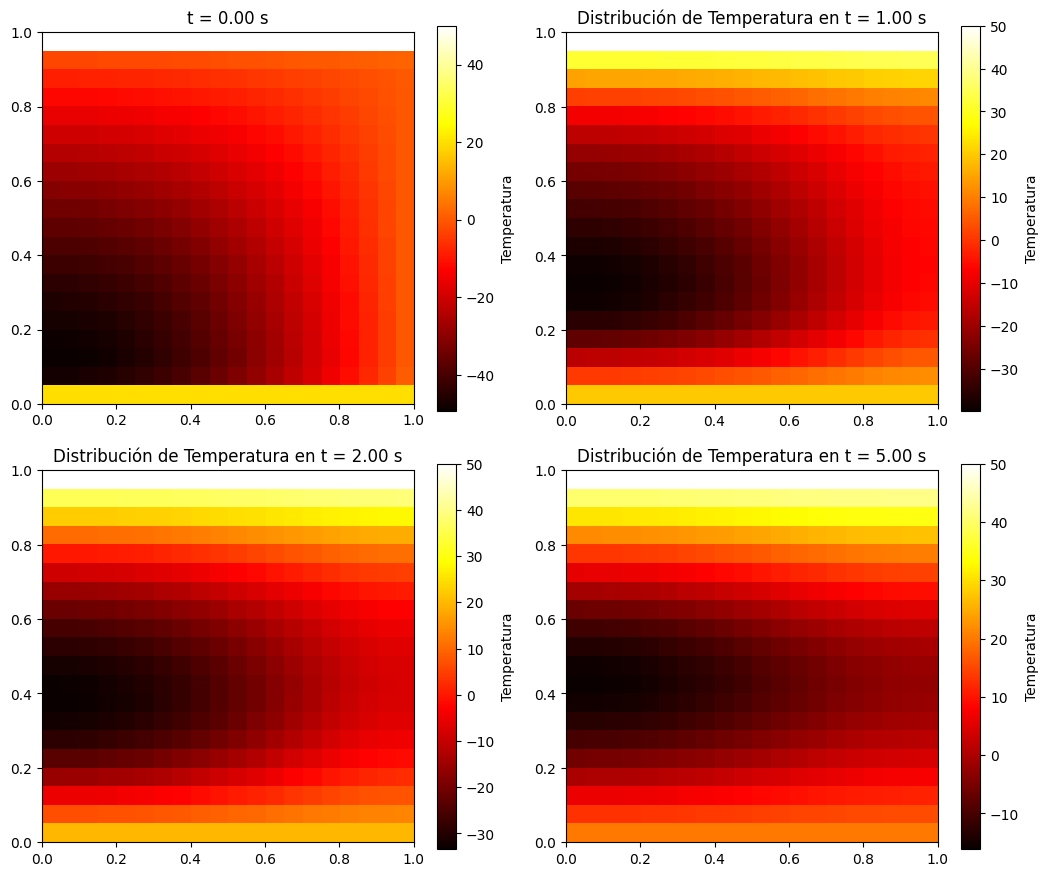
\includegraphics[width=0.58\textwidth]{img/tiempos_st.jpg}
    \caption{Evolución de la distribución de temperatura para $t = 0$, $1.0$, $2.0$ y $5.0$ segundos.}
    \label{fig:temp_times}
\end{figure}

El método implícito empleado garantiza \textbf{estabilidad incondicional} en cada iteración temporal, lo que permite avanzar en el tiempo con pasos relativamente amplios sin degradar la solución. Gracias a la discretización en diferencias finitas centradas en espacio y hacia atrás en tiempo, se asegura la convergencia del esquema, hecho que se refleja en la progresiva suavización del perfil térmico hacia una distribución estable.\\

Desde el punto de vista numérico, se aprecia cómo la influencia de las condiciones de Dirichlet en los bordes superior e inferior se propaga hacia el interior del dominio, mientras que los bordes verticales con condiciones de Neumann mantienen una gradiente nula, respetando la simetría térmica esperada. Este fenómeno de difusión es característico de las ecuaciones parabólicas y valida el comportamiento físico simulado.\\

La evolución del sistema sigue una lógica coherente con la teoría de estabilidad térmica: en tiempos intermedios, se mantiene una transición activa del gradiente térmico, mientras que para tiempos prolongados la solución tiende hacia un régimen estacionario. Este resultado confirma que el método numérico no solo es estable y consistente, sino que también reproduce fielmente el fenómeno físico modelado.\\


\noindent Los efectos de la difusión térmica observados en esta simulación serán objeto de un análisis más detallado en el apartado de \textbf{Discusión} (ver Sección~\ref{subsubsec:dt}), dónde se abordará la interpretación cualitativa y cuantitativa del comportamiento del sistema.

\subsubsection{Estudio de convergencia espacial.}
Para evaluar la consistencia y precisión del esquema numérico implementado, se ha llevado a cabo un estudio de convergencia espacial analizando el valor de la temperatura en el punto central del dominio en el instante $t = 5$ segundos. Se han considerado distintos tamaños de mallado uniformes: $N = 10$, $20$, $40$, $50$, $60$ y $80$, manteniendo fijo el valor del parámetro $\lambda = \alpha \Delta t / h^2$ para garantizar condiciones de estabilidad homogéneas.\\

En la Figura~\ref{fig:convergencia} se observa cómo el valor de temperatura en el centro converge de forma monótona a medida que se refina el mallado. Los resultados reflejan una mejora sustancial de la precisión al incrementar la resolución espacial, especialmente en las primeras refinaciones. A partir de $N = 50$, la diferencia entre iteraciones consecutivas se reduce significativamente, lo que indica una estabilización del valor numérico hacia una \textbf{solución asintótica}.\\

Este comportamiento evidencia que el esquema utilizado presenta propiedades de consistencia y convergencia adecuadas, cumpliendo los requisitos teóricos para ecuaciones parabólicas. Además, la elección del punto central como referencia es especialmente significativa, ya que es una \textbf{zona influida por todas las condiciones de contorno y por tanto altamente representativa} del comportamiento global de la solución.

\begin{figure}[H]
    \centering
    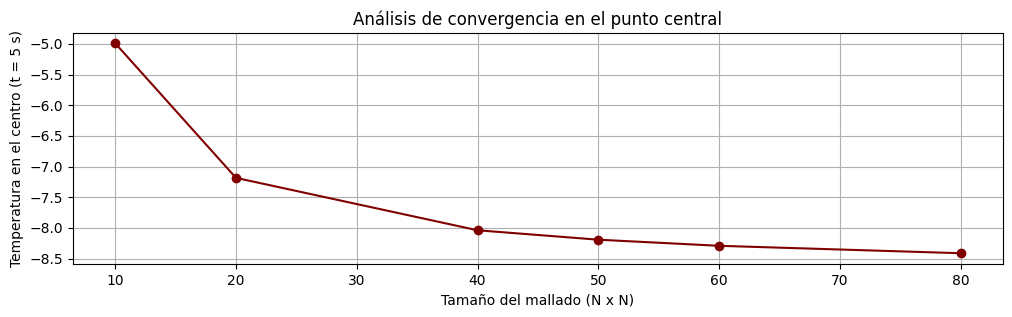
\includegraphics[width=0.62\textwidth]{img/convergencia.png}
    \caption{Análisis de convergencia en el centro del dominio para $t=5$ s y diferentes tamaños de malla.}
    \label{fig:convergencia}
\end{figure}

\subsubsection{Comparativa Visual entre Mallados.}
Para ilustrar el efecto del refinamiento espacial en la calidad de la solución numérica, se presentan a continuación las distribuciones de temperatura obtenidas en el instante $t = 5$ segundos para tres configuraciones de malla: $10 \times 10$, $20 \times 20$ y $40 \times 40$. Las imágenes térmicas correspondientes se muestran en la Figura~\ref{fig:mallados}.

\begin{figure}[H]
    \centering
    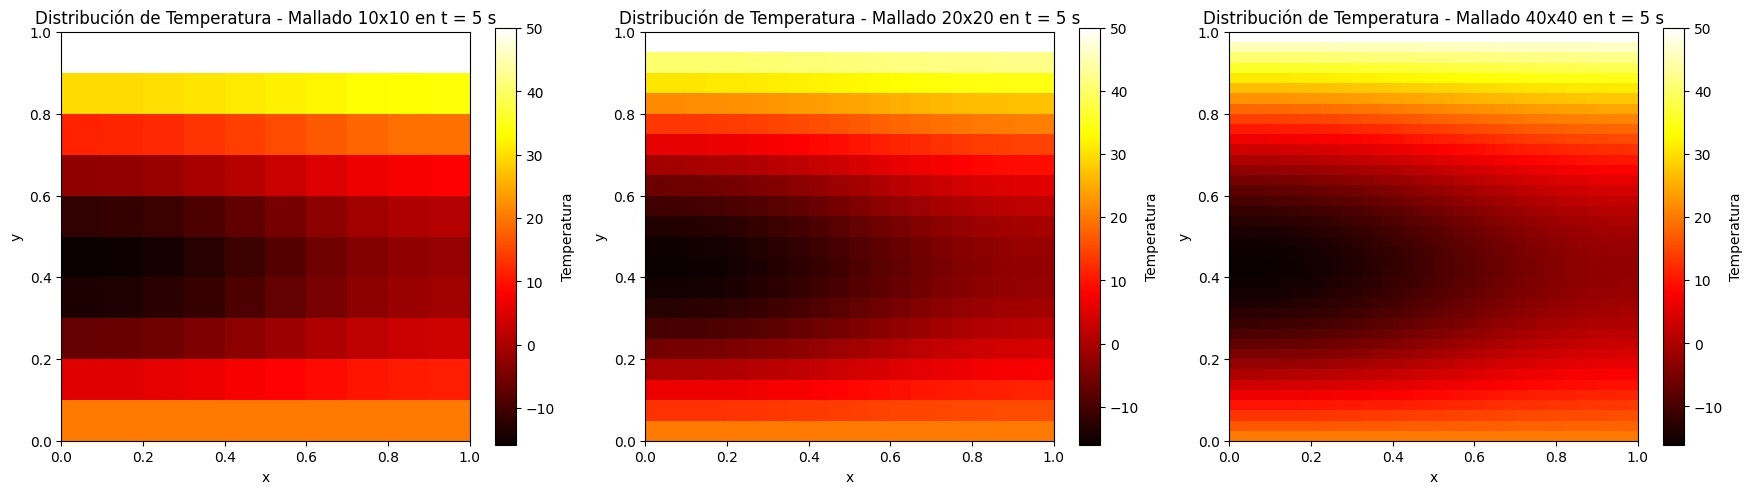
\includegraphics[width=0.9\textwidth]{img/mallados_st.jpg}
    \caption{Distribución de temperatura para $t = 5$ s con mallados $10 \times 10$, $20 \times 20$ y $40 \times 40$.}
    \label{fig:mallados}
\end{figure}

La comparación evidencia una \textbf{clara mejora en la resolución de los gradientes térmicos conforme se incrementa la densidad del mallado}. En la malla más gruesa ($10 \times 10$), los contornos térmicos aparecen pixelados y con baja definición, dificultando la interpretación precisa de la distribución. En cambio, las simulaciones con $20 \times 20$ y especialmente $40 \times 40$ muestran transiciones suaves y bien definidas entre zonas de distinta temperatura, lo cual permite representar con mayor fidelidad los fenómenos físicos subyacentes.\\

Desde una perspectiva de simulación numérica, este análisis visual corrobora los resultados del estudio de convergencia: el refinamiento espacial no solo \textbf{mejora la precisión de los valores puntuales}, sino también la \textbf{calidad visual e interpretativa de la solución global}. Sin embargo, se debe tener en cuenta que el aumento de resolución conlleva un \textbf{incremento en el coste computacional}, tanto en términos de memoria como de tiempo de cálculo. En este caso, el uso de \textbf{matrices dispersas ha permitido gestionar dicho coste de forma eficiente}, posibilitando la simulación con mallados relativamente densos sin comprometer la viabilidad computacional.\\

\noindent
El análisis más detallado de la influencia del mallado en la calidad de la simulación y en la interpretación física de la solución será retomado y ampliado en el apartado de \textbf{Discusión} (ver Sección~\ref{subsubsec:dt}).

\newpage
\subsection{Simulación Estacionaria: Resolución con Matrices Dispersas en Formato CSR Manual.}
\label{subsubsec:re}
En esta sección se presentan los resultados correspondientes a la resolución de la ecuación del calor en estado estacionario, es decir, cuando el sistema alcanza una configuración térmica estable y las derivadas temporales desaparecen. Para ello, se ha considerado la forma elíptica de la ecuación, que implica resolver un sistema lineal derivado de la discretización espacial mediante diferencias finitas.\\

A diferencia de la parte transitoria, en este caso la matriz del sistema ha sido construida manualmente en formato disperso comprimido por filas (\texttt{CSR}), sin el uso de librerías externas. Esta elección permite un control completo sobre la estructura y el ensamblado del sistema lineal, lo que resulta de especial interés desde el punto de vista didáctico y computacional.\\

Con el objetivo de analizar la influencia del mallado en la precisión y estabilidad de la solución, se han considerado diferentes discretizaciones: mallas gruesas de $10 \times 10$ y mallas más refinada tales como $40 \times 40$. Para ambas configuraciones se representa la distribución térmica final en el dominio, analizando el efecto de las condiciones de contorno y comparando los resultados con los obtenidos al final del régimen transitorio.

\subsubsection{Distribución térmica estacionaria.}
En la Figura~\ref{fig:estacionaria20} se muestra la solución obtenida para el régimen estacionario utilizando una discretización de $20 \times 20$ nodos interiores. El perfil térmico resultante se caracteriza por una transición progresiva desde los $20^\circ$C en el borde inferior hasta los $50^\circ$C en el borde superior del dominio. La distribución es suave, sin oscilaciones ni discontinuidades, lo cual valida tanto la implementación numérica como la formulación física del problema.\\

Se observa que el gradiente de temperatura se mantiene prácticamente uniforme en la dirección vertical, mientras que en la dirección horizontal las variaciones son despreciables, como era esperable dadas las condiciones de contorno homogéneas de tipo Neumann impuestas en los laterales. Este comportamiento confirma que la solución obtenida corresponde a un estado de equilibrio térmico, dónde la difusión ha alcanzado un régimen constante en todo el dominio.

\begin{figure}[H]
    \centering
    
\includegraphics[width=0.52\textwidth]{img/estacionaria_sparse.png}
    \caption{Distribución estacionaria de temperatura para mallado $20 \times 20$.}
    \label{fig:estacionaria20}
\end{figure}

\noindent
Este resultado es coherente con la evolución observada en la simulación transitoria, en la cual se anticipaba una estabilización en torno al perfil aquí mostrado. El análisis detallado de la calidad de esta solución, su convergencia y su comparativa con otros mallados será abordado en profundidad en el apartado de \textbf{Discusión} (ver Sección~\ref{subsubsec:de}).

\subsubsection{Comparación Visual entre Mallados.}

Con el objetivo de evaluar el efecto del refinamiento espacial en la calidad de la solución estacionaria, se ha comparado la distribución de temperatura obtenida con tres tamaños de malla: $10 \times 10$, $20 \times 20$ y $40 \times 40$. Las soluciones correspondientes se muestran en la Figura~\ref{fig:comparativa_mallados}.

\begin{figure}[H]
    \centering
    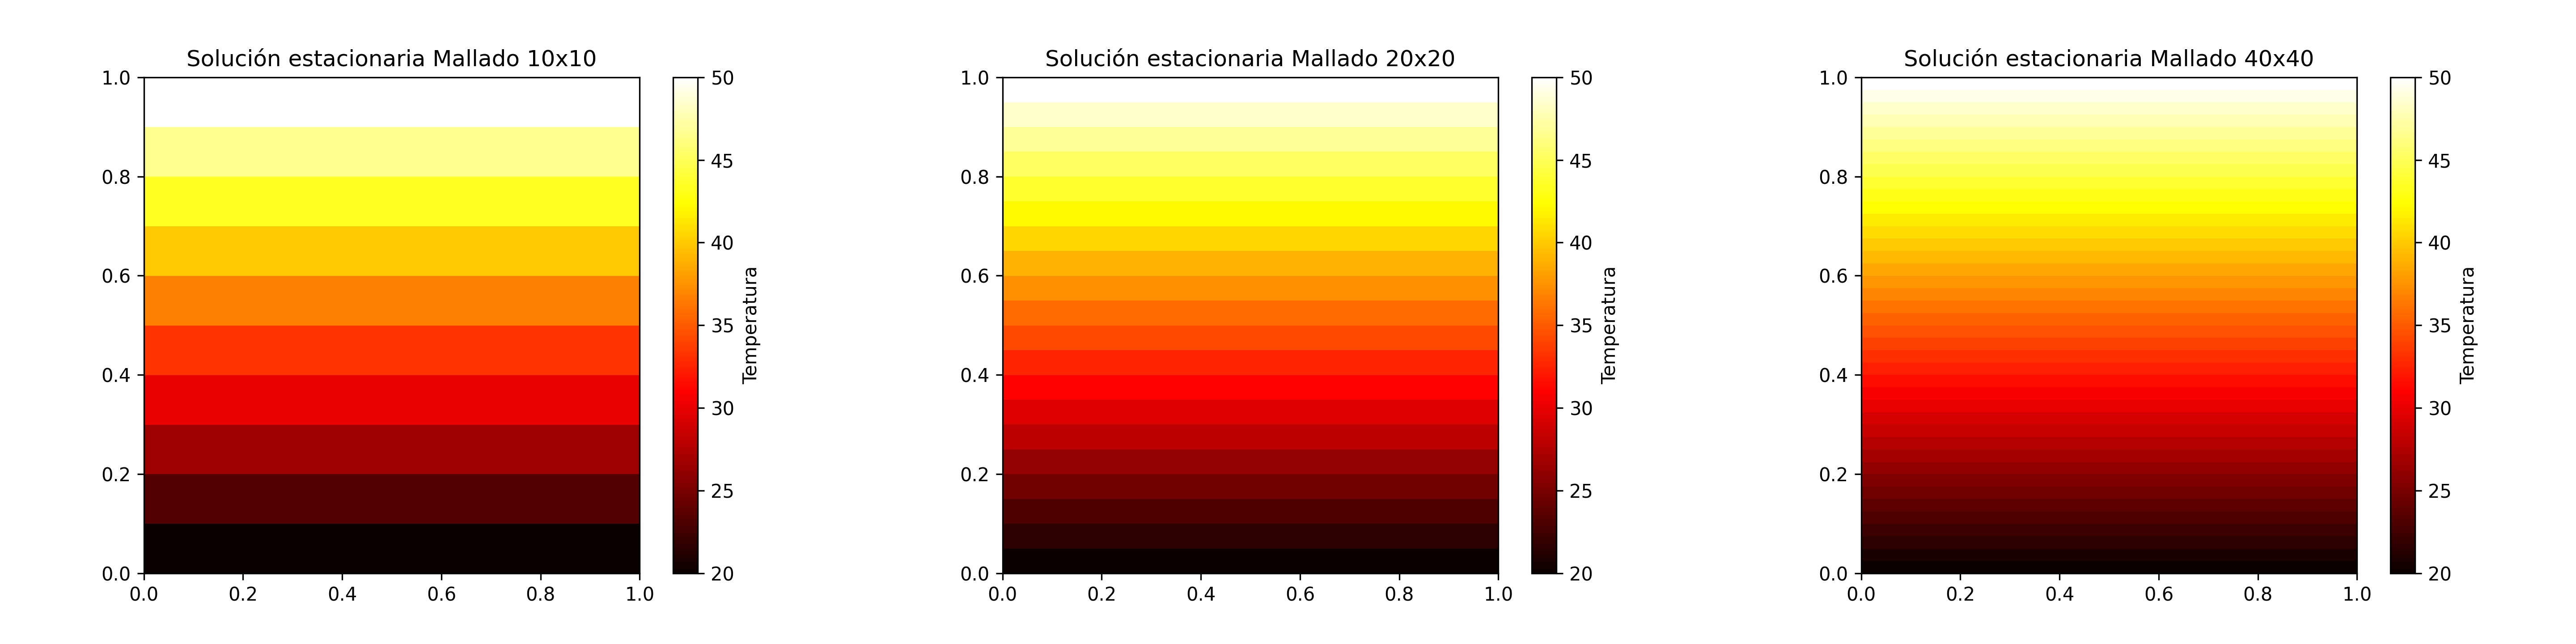
\includegraphics[width=1\textwidth]{img/mallados_se.jpg}
    \caption{Distribución de temperatura para mallados $10 \times 10$, $20 \times 20$ y $40 \times 40$.}
    \label{fig:comparativa_mallados}
\end{figure}

La comparación revela que el \textbf{mallado más grueso} ($10 \times 10$) presenta una \textbf{estructura escalonada}, con franjas térmicas que \textbf{carecen de continuidad entre celdas}. Aunque refleja la tendencia general del sistema, la precisión visual y numérica es limitada. En el \textbf{mallado intermedio} ($20 \times 20$), se observa una \textbf{mejora notable} en la suavidad de los gradientes térmicos, lo que permite una representación más precisa del equilibrio térmico esperado.\\

El \textbf{mallado más fino} ($40 \times 40$) ofrece una \textbf{solución muy próxima al perfil ideal continuo}, con una transición térmica suave y homogénea a lo largo del dominio. No obstante, este incremento de resolución implica también un \textbf{mayor coste computacional} y una complejidad adicional en la gestión de estructuras dispersas, especialmente cuando se trabaja sin librerías externas.\\

\noindent En términos generales, puede concluirse que la malla $20 \times 20$ ofrece un equilibrio adecuado entre precisión y coste, mientras que el mallado $40 \times 40$ sería preferible en aplicaciones que requieran mayor detalle local. El análisis cualitativo y cuantitativo más detallado de estas diferencias se desarrollará en el apartado de \textbf{Discusión} (ver Sección~\ref{subsubsec:de}).



%DISCUSIÓN
\newpage
\section{Discusión.}
\subsection{Evaluación del Régimen Transitorio.}
\label{subsubsec:dt}
\paragraph{Interpretación física de la evolución térmica.} La simulación del régimen transitorio ha permitido observar de forma clara y coherente el fenómeno de difusión térmica a lo largo del dominio. La \textbf{evolución desde un perfil inicial de temperatura negativo hacia un estado más uniforme} responde fielmente a la dinámica esperada en sistemas gobernados por ecuaciones en derivadas parciales parabólicas. Las condiciones de contorno mixtas han tenido un impacto determinante: las fronteras horizontales con valores fijos imponen gradientes térmicos relevantes, mientras que los bordes verticales con condiciones de Neumann permiten mantener un equilibrio simétrico sin intercambio de calor.\\

El sistema muestra una clara \textbf{relajación hacia el equilibrio}, y en torno a $t=5$ segundos la solución comienza a estabilizarse. Este comportamiento valida tanto la formulación física del problema como su implementación numérica, y anticipa la convergencia hacia el régimen estacionario que se analizará posteriormente (ver Sección~\ref{subsubsec:re}.

\paragraph{Robustez y estabilidad del método implícito.} El método implícito utilizado ha demostrado ser especialmente robusto para este tipo de simulaciones. La \textbf{estabilidad incondicional} del esquema ha permitido utilizar \textbf{pasos temporales relativamente amplios sin introducir inestabilidades numéricas}. Esto se refleja en la ausencia de oscilaciones espurias y en la suavidad de los perfiles de temperatura obtenidos a lo largo del tiempo.\\

El uso de matrices dispersas en formato \texttt{CSR} mediante la biblioteca \texttt{scipy.sparse} ha sido clave para mantener un coste computacional razonable incluso en simulaciones con mallas relativamente finas. Este enfoque permite escalar el modelo a resoluciones más altas sin comprometer recursos, lo que resulta especialmente útil en entornos de simulación aplicados.\\

No obstante, la formulación implícita conlleva también ciertos desafíos. El ensamblado y resolución de un sistema lineal en cada paso de tiempo introduce una \textbf{carga computacional considerable}, sobre todo para mallados grandes. En simulaciones más exigentes o tridimensionales, podría ser necesario recurrir a métodos iterativos precondicionados o técnicas multigrid para mantener la eficiencia.

\paragraph{Convergencia espacial y validación numérica.} El análisis de convergencia en el punto central ha evidenciado una \textbf{mejora progresiva de la precisión} a medida que se refina el mallado. Los resultados numéricos muestran una \textbf{convergencia monótona hacia un valor límite}, lo que confirma que el esquema de discretización es tanto consistente como convergente. Esta propiedad es fundamental en la validación de cualquier método numérico aplicado a ecuaciones diferenciales parciales.\\

La elección del valor en el nodo central como referencia ha sido adecuada, ya que dicho punto sintetiza las influencias de las distintas condiciones de contorno y permite evaluar la calidad global de la solución.\\

Sin embargo, se ha observado que a partir de un cierto umbral de refinamiento (en torno a $N=50$), las ganancias en precisión son mínimas en relación al incremento del coste computacional. Esto pone de manifiesto la necesidad de establecer \textbf{criterios de parada o selección óptima del mallado} en función del objetivo de la simulación.

\paragraph{Impacto del mallado en la representación física.} La comparación visual entre las soluciones obtenidas con distintos tamaños de malla revela de forma clara el impacto del refinamiento espacial en la calidad de la simulación. Mientras que las \textbf{mallas más gruesas} ($10 \times 10$) presentan \textbf{contornos pixelados y escasa resolución} de gradientes, las \textbf{mallas más densas} ($20 \times 20$, $40 \times 40$) logran capturar \textbf{transiciones térmicas suaves y más representativas} del fenómeno físico real.\\

Este resultado no solo justifica la elección de un mallado adecuado para cada tipo de estudio, sino que también demuestra la \textbf{efectividad del tratamiento numérico del problema} y la correcta implementación de las condiciones de contorno. Asimismo, permite establecer un equilibrio entre precisión y coste computacional, optimizando el rendimiento de la simulación sin sacrificar fidelidad física.

\paragraph{Transición hacia el régimen estacionario.} La estabilización observada en los últimos instantes simulados sugiere que el sistema ha alcanzado, o está muy próximo a alcanzar, su configuración estacionaria. Esto abre la puerta a una comparación directa con la solución obtenida en régimen permanente, que será abordada en el siguiente apartado. Dicha comparación permitirá validar la precisión del esquema implícito en el largo plazo y establecer la coherencia global del modelo.


\subsection{Evaluación del Régimen Estacionario.}
\label{subsubsec:de}
\paragraph{Coherencia física de la solución.} Los resultados obtenidos para el régimen estacionario \textbf{reflejan con precisión el comportamiento esperado} de un sistema difusivo en equilibrio térmico. La distribución de temperatura muestra un \textbf{gradiente prácticamente lineal en dirección vertical}, con contornos paralelos que conectan las condiciones de contorno fijas (Dirichlet) impuestas en los bordes superior e inferior. La ausencia de variación significativa en dirección horizontal confirma que las condiciones de Neumann homogéneas han sido correctamente implementadas.\\

Esta solución está en completa concordancia con la configuración física planteada: en ausencia de fuentes internas, y con condiciones constantes en los bordes, el sistema tiende hacia una solución estable que minimiza los gradientes térmicos, de forma coherente con la ecuación. \\

Sin embargo, al trabajar con una malla uniforme y cartesianamente estructurada, se limita la posibilidad de adaptar localmente la resolución a zonas con mayores variaciones térmicas. Esto puede ser un inconveniente en problemas reales más complejos, donde la geometría del dominio o las fuentes de calor no estén uniformemente distribuidas.

\paragraph{Validación mediante comparación con la solución transitoria.} Uno de los aspectos más relevantes de este apartado ha sido la comparación de la solución estacionaria con el comportamiento del modelo en régimen transitorio. Tal como se observó en la sección anterior, al alcanzar $t = 5$ segundos, el perfil térmico generado por la simulación transitoria comenzaba a estabilizarse hacia una distribución equivalente a la obtenida aquí.\\

Esta correspondencia valida de forma cruzada ambas implementaciones: la estabilidad alcanzada en el tiempo largo en la fase transitoria y la precisión de la solución directa en régimen estacionario. El hecho de que \textbf{ambas converjan a una misma distribución fortalece la consistencia numérica del modelo.}


\paragraph{Influencia del mallado y resolución de gradientes.} La comparación entre mallados ($10 \times 10$, $20 \times 20$ y $40 \times 40$) ha permitido evidenciar el impacto directo de la resolución espacial sobre la calidad visual y numérica de la solución. Si bien todos los casos reflejan el comportamiento térmico global, solo los \textbf{mallados más refinados son capaces de capturar transiciones suaves y representar adecuadamente el gradiente}.\\

El \textbf{mallado intermedio} ($20 \times 20$) se ha confirmado como un \textbf{punto de equilibrio} entre \textbf{precisión} y \textbf{coste computacional}, especialmente relevante en un contexto donde \textbf{no se han utilizado librerías externas para gestionar estructuras dispersas}. Por otro lado, el mallado $40 \times 40$ presenta mejoras visuales, pero con un coste de implementación mayor, que podría volverse prohibitivo en mallas más grandes si no se automatiza el ensamblado o resolución del sistema.

\paragraph{Resolución del sistema y eficiencia numérica.} Una limitación relevante ha sido la ausencia de un análisis cuantitativo del error asociado a cada mallado, por ejemplo, mediante norma $L^2$ o comparación con una solución analítica. Esta evaluación permitiría establecer de forma objetiva la ganancia real obtenida al refinar la malla, y definir criterios numéricos de parada o de tolerancia.\\

Además, la resolución del sistema lineal se ha realizado mediante \textbf{métodos directos básicos}. En simulaciones más complejas o tridimensionales, sería necesario recurrir a \textbf{algoritmos iterativos más eficientes}, o integrar técnicas multigrid si se desea mantener la escalabilidad.

\newpage
\section{Conclusiones.}
 A lo largo de este trabajo se ha abordado la resolución numérica de la ecuación del calor en dos dimensiones, bajo condiciones de contorno mixtas y mediante la aplicación del método de diferencias finitas implícito. El desarrollo se ha estructurado en dos fases diferenciadas: una primera orientada a la simulación en régimen transitorio, utilizando estructuras dispersas proporcionadas por la biblioteca \texttt{Scipy}; y una segunda, centrada en el régimen estacionario, donde se ha implementado de forma manual la estructura \texttt{CSR} sin apoyo de librerías externas.\\

En la fase transitoria, se ha logrado una representación realista de la evolución térmica del sistema, verificando la estabilidad y precisión del método implícito incluso para pasos de tiempo amplios. La evolución hacia el equilibrio ha sido coherente con el comportamiento físico esperado, y el análisis de convergencia ha demostrado que el refinamiento espacial mejora significativamente la precisión de los resultados. La implementación con matrices dispersas ha permitido optimizar el rendimiento computacional, haciendo viable la simulación con mallas densas.\\

En la fase estacionaria, la implementación manual del formato CSR ha evidenciado tanto su validez matemática como sus limitaciones prácticas. Se ha verificado que la solución obtenida es coherente con el estado final del sistema transitorio, reforzando así la consistencia global del modelo. No obstante, la construcción artesanal de la matriz y la resolución mediante algoritmos directos básicos presentan una escalabilidad limitada, poco adecuada para dominios grandes o geometrías complejas.\\

Desde un punto de vista didáctico, el trabajo ha permitido profundizar en los fundamentos de la simulación numérica, el manejo de estructuras dispersas, y el análisis crítico de resultados. Sin embargo, también ha dejado de manifiesto la necesidad de automatización, validación cuantitativa y uso de métodos numéricos avanzados para poder abordar simulaciones más realistas o exigentes.\\

Como línea de mejora futura, se propone extender el modelo a geometrías irregulares, incorporar fuentes térmicas internas, y emplear esquemas adaptativos en malla y tiempo. Asimismo, el uso de precondicionadores y técnicas iterativas avanzadas permitiría escalar el modelo a contextos industriales o científicos reales.\\

En definitiva, se ha logrado una implementación completa, funcional y técnicamente coherente del método implícito en régimen transitorio y estacionario, combinando rigor numérico y comprensión profunda de las limitaciones del enfoque empleado.


%REFERENCIAS
\newpage
\section{Referencias.}
\renewcommand{\refname}{}
\renewcommand{\bibname}{}
\vspace{-10mm}
\begin{thebibliography}{99}

% Introducción a la ecuación de calor
\bibitem{intro_calor1} Wikipedia. (s.f.). \textit{Ecuación del calor}. Recuperado de \url{https://es.wikipedia.org/wiki/Ecuaci%C3%B3n_del_calor}

\bibitem{intro_calor2} Iglesias Díaz, A. (2022). \textit{La ecuación del calor}. Universidad de Barcelona. Recuperado de \url{https://diposit.ub.edu/dspace/bitstream/2445/211361/1/tfg_iglesias_diaz_angel.pdf}

% Solución transitoria
\bibitem{transitoria1} Universidad de Murcia. (2020). \textit{La ecuación del calor}. Recuperado de \url{https://webs.um.es/gustavo.garrigos/tfg/Milonga_TFG_sept2020.pdf}

% Método explícito
\bibitem{explicito1} Ginestar, D. (2022). \textit{Prácticas de métodos numéricos para ecuaciones en derivadas parciales}. Universitat Politècnica de València. Recuperado de \url{https://personales.upv.es/dginesta/docencia/posgrado/prac_intro_edps.pdf}


% Método implícito
\bibitem{implicito1} Universidad de Zaragoza. (s.f.). \textit{Método de Crank-Nicolson}. Recuperado de \url{https://www.ugr.es/~prodelas/ftp/ETSICCP/Resoluci%F3nNum%E9ricaEDPs.pdf}

\bibitem{implicito2} Universidad Politécnica de Cartagena. (s.f.). \textit{Tema 7: Método de diferencias finitas}. Recuperado de \url{https://www.dmae.upct.es/~paredes/calcnum/apuntes/apuntes_tema_7.pdf}

% Método implícito con matrices sparse (transitorio)
\bibitem{sparse_trans1} Universitat Politècnica de Catalunya (UPC). (2016). \textit{Solución numérica de la ecuación del calor utilizando matrices sparse}. Recuperado de \url{https://upcommons.upc.edu/bitstream/handle/2117/94028/01MLss01de04.pdf}


% Solución estacionaria
\bibitem{estacionaria1} Universidad de la República (Uruguay). (s.f.). \textit{Introducción a la ecuación de calor estacionaria}. Recuperado de \url{https://eva.fing.edu.uy/pluginfile.php/253661/mod_resource/content/4/Capitulo1_introduccion.pdf}

% Método implícito estacionario
\bibitem{est_implicito1} Universidad de La Laguna. (s.f.). \textit{Métodos numéricos para la resolución de ecuaciones diferenciales y aplicaciones}. Recuperado de \url{https://riull.ull.es/xmlui/bitstream/handle/915/16290/Metodos%20numericos%20para%20la%20resolucion%20de%20ecuaciones%20diferenciales%20y%20aplicaciones..pdf?sequence=1&isAllowed=y}

% Método implícito con matrices sparse (estacionario)
\bibitem{est_sparse1} Universidad de Barcelona. (2017). \textit{Modelización de la ecuación de calor con diferencias finitas}. Recuperado de \url{https://diposit.ub.edu/dspace/bitstream/2445/122103/2/memoria.pdf}

\end{thebibliography}


%ANEXOS
\newpage
\section{Anexos.}
El código fuente de estas implementaciones está disponible en el siguiente repositorio de GitHub:  
\href{https://github.com/mgonzalz/sn_talleres/blob/main/notebooks/informe-02__ecuacion-calor.ipynb}{\texttt{GitHub - mgonzalz/sn\_talleres}}.
\subsection{Resolución Transitoria: Evolución Térmica en el Tiempo.}
Este script simula la evolución temporal de la temperatura en una placa 2D sujeta a condiciones de contorno mixtas. Se utiliza un esquema implícito estable que genera un sistema lineal en cada paso de tiempo, resuelto mediante \texttt{spsolve()} sobre una matriz dispersa en formato \texttt{CSC}. Se incorporan condiciones de Dirichlet en la parte superior e inferior, y Neumann en los laterales. Además, se genera una animación visual de la distribución térmica a lo largo del tiempo.

\lstinputlisting[style=python, caption=Simulación Transitoria de la Ecuación de Calor con Matriz Sparse y Esquema Implícito.]{python/transitoria.py}

\newpage
\subsection{Resolución Estacionaria: Método Directo en Régimen Estático.}
Este script implementa la solución en estado estacionario de la ecuación de calor en 2D, utilizando diferencias finitas centradas. Se construye una matriz dispersa en formato \texttt{CSR} respetando condiciones de contorno mixtas: Dirichlet en los extremos verticales y Neumann en los laterales. El sistema resultante se resuelve mediante el método iterativo de \textbf{Gauss-Seidel} aplicado directamente al formato disperso, optimizando la memoria y el tiempo de cálculo.

\lstinputlisting[style=python, caption=Resolución Estacionaria de la Ecuación de Calor con Condiciones de Dirichlet y Neumann.]{python/estacionaria.py}

\end{document}
